% !TeX root = ../main.tex

\chapter{Theory}

%\section{The Standard Model of Particle Physics}
\section{Elementary Particles and Interactions in the Standard Model}
The standard model (SM) reflects our current understanding of elementary particles and several basic interactions.
It is a gauge quantum field theory containing the internal symmetries of the unitary product group $SU(3) \times SU(2) \times U(1)$, 
in which the color group $SU(3)$ presents the strong interaction, and $SU(2) \times U(1)$ describes the electroweak interactions.
Over the past decades, the SM has been widely tested through various experiments with extremely high precision.

\subsection{Elementary particles in the Standard Model}
\label{elementaryparticles}

The elementary particles in SM can be classified into 3 class: \textit{fermions}, \textit{gauge bosons} and the \textit{Higgs boson} as shown in Figure~\ref{fig:eleP-1}.
\begin{figure}[!htb]
  \centering
  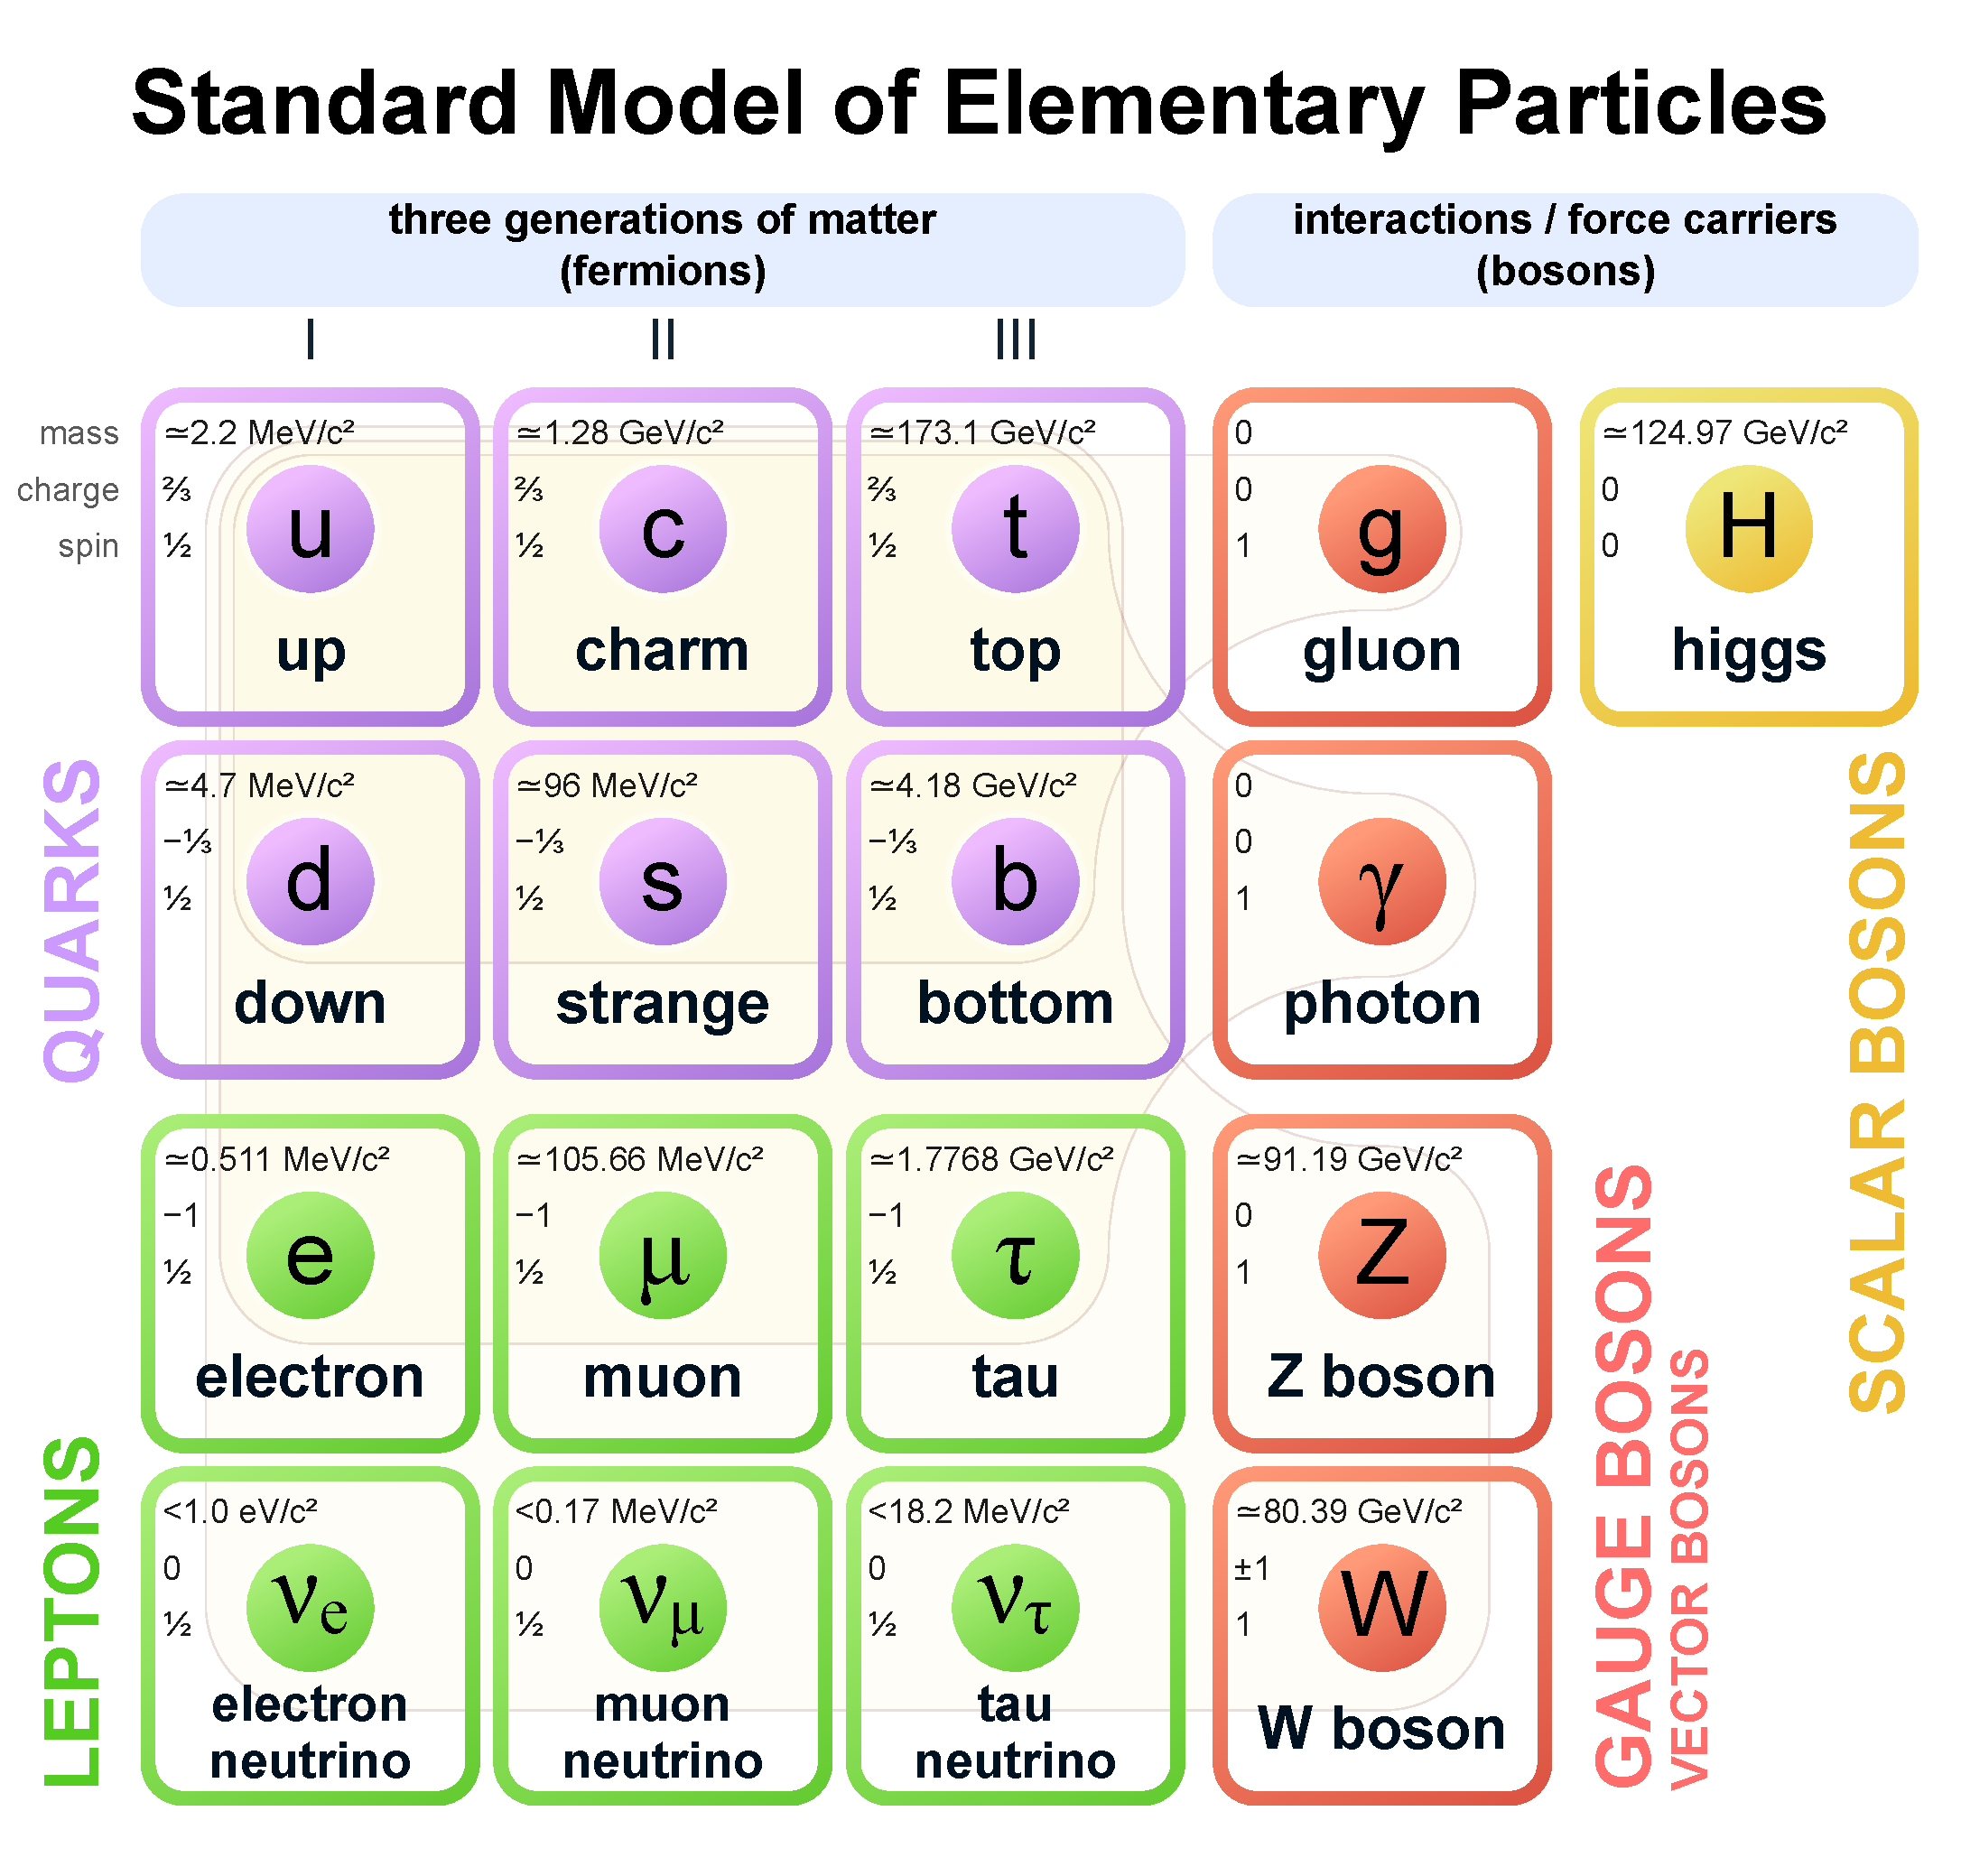
\includegraphics[width=0.7\textwidth]{figures/Theory/Standard_Model_of_Elementary_Particles.pdf}
  \caption{The elementary particles of the Standard Model.}
  \label{fig:eleP-1}
\end{figure}

\textbf{Fermions}
The Standard Model includes 12 elementary particles of spin-$\frac{1}{2}$ obeying the Fermy-Dirac statistics, known as fermions. 
They are classified into two types: \textit{leptons} and \textit{quarks} according to the their interactions.
The \textit{leptons} include three generations: electron ($e$) and electron neutrino ($\nu_{e}$); 
muon ($\mu$) and muon neutrino ($\nu_{\mu}$); tau ($\tau$) and tau neutrino ($\nu_{\tau}$).
The $e$, $\mu$ and $\tau$ carry electric charge of -1 and three neutrinos are electrically neutral. 
All the leptons can participate in electroweak interactions.
Also there are three generations of \textit{quarks}: up ($u$) and down ($d$); charm ($c$) and strange ($s$); top ($t$) and bottom ($b$).
The defining property of the quarks is that they carry color charge (while leptons don't), and hence interact via the strong interaction, 
letting them to be strongly bound from one to another, forming color-neutral composite 
particles (known as hadrons) containing either a quark and an antiquark (mesons) or three quarks (baryons).
In the meantime, $u$, $c$ and $t$ -quark carry electric charge of 2/3, and $d$, $s$ and $b$ -quark carry electric charge of -1/3. 
Hence they interact via all three interactions described in SM.
Each fermion also has its corresponding antiparticle.

\textbf{Gauge bosons}
act as force carriers that propagate the strong, weak, and electromagnetic interactions in SM.
They are spin-1 particles obeying the Bose-Einstein statistics. 
There are three types of gauge bosons:
\begin{itemize}
  \item The eight massless \textit{gluons} propagate the strong interactions between color charged particles (quarks).
  \item The massless \textit{photons} propagate the electromagnetic force between electrically charged particles.
  \item The $W^{+}$, $W^{-}$ and $Z$ bosons propagate the weak interactions between both quarks and leptons. All these three bosons are massive, the $W^{\pm}$ carries an electric charge of $+1$ and $−1$ and can also couple to the electromagnetic interaction while $Z$ boson is electrically neutral.
\end{itemize}
Figure~\ref{fig:eleP-2} shows the Feynman diagrams of corresponding interactions in SM.
\begin{figure}[!htb]
  \centering
  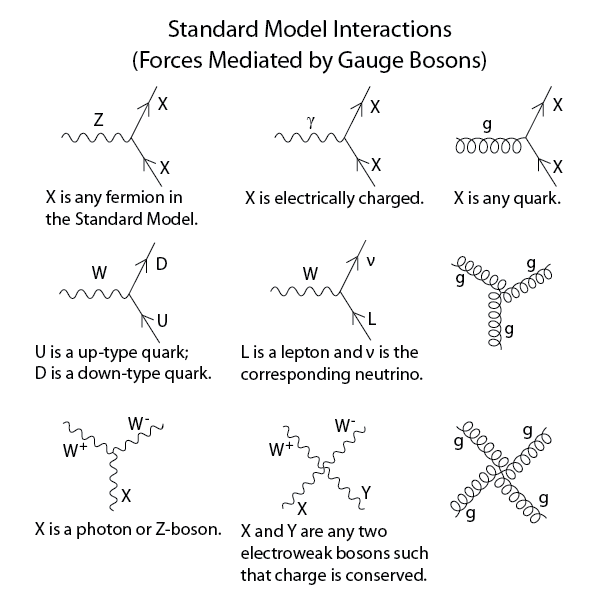
\includegraphics[width=0.8\textwidth]{figures/Theory/Standard_Model_Feynman_Diagram_Vertices.png}
  \caption{The Feynman diagrams of interactions mediated by gauge bosons that form the basis of the standard model.}
  \label{fig:eleP-2}
\end{figure}

\textbf{Higgs boson}
is a massive scaler elementary particle with spin-0. 
It plays a unique role in the SM by explaining the origin of masses of massive gauge bosons ($W^{\pm} and Z$) and fermions. 
And it is the last discovered particle in SM.

%\subsection{Elementary particles in the Standard Model}
\subsection{Electroweak theory}
\label{ewktheory}
The electroweak interaction is the unified description of two of the four known fundamental interactions of nature: electromagnetism and the weak interaction.
It is based on the gauge group of $SU(2)_{L} \times SU(1)_{Y}$, in which $L$ is the left-handed fields and $Y$ is the weak hypercharge \cite{Langacker:2009my}.
It follows the Lagrangian of
\begin{equation} \label{eq:Lew}
	L_{EW} = L_{gauge} + L_{Higgs} + L_{fermion} + L_{Yukawa}
\end{equation}

$L_{gauge}$ is the \textbf{gauge term} part
\begin{equation}
	L_{gauge} = -\frac{1}{4} W^{i}_{\mu\nu} W^{\mu\nu i} - \frac{1}{4} B_{\mu\nu} B^{\mu\nu}
\end{equation}
where $W^{i}_{\mu}$ and $B_{\mu}$ respectively present the $SU(2)_{L}$ and $SU(1)_{Y}$ gauge fields, with the corresponding field strength tensors of
\begin{equation}
\begin{split}
	& B_{\mu\nu} = \partial_{\mu} B_{\nu} - \partial_{\nu} B_{\mu} \\
	& W^{i}_{\mu\nu} = \partial_{\mu} W^{i}_{\nu} - \partial_{\nu} W^{i}_{\mu} - g \epsilon_{ijk} W^{j}_{\mu} W^{k}_{\nu}
\end{split}
\end{equation}
In the equations above, $g$ is the $SU(2)_{L}$ gauge coupling and $\epsilon_{ijk}$ is the totally antisymmetric tensor.
The gauge Lagrangian has three and four-point self interactions of $W^{i}$, which result in triple and quartic gauge boson couplings.

The second term of the Lagrangian is the \textbf{scaler part}:
\begin{equation} \label{eq:Lhiggs}
	{L}_{Higgs} = \left(D^{\mu}\phi\right)^{\dagger}D_{\mu}\phi - V(\phi)
\end{equation}
where $\phi = \binom{\phi^{+}}{\phi^{0}}$  is a complex Higgs scalar,
and $V(\phi)$ is the Higgs potential which is restricted into the form of 
\begin{equation} \label{eq:Vhiggs}
	V(\phi) = +\mu^{2}\phi^{\dagger}\phi + \lambda\left(\phi^{\dagger}\phi\right)^{2}
\end{equation}
due to the combination of $SU(2)_{L} \times SU(1)_{Y}$ invariance and renormalizability.
In Eq.~\ref{eq:Vhiggs}, $\mu$ is a mass-dependent parameter and $\lambda$ is the quartic Higgs scalar coupling, 
which represents a quartic self-interaction between the scalar fields.
When $\mu^{2} < 0$, there will be spontaneous symmetry breaking (more details in section~\ref{symbreaking}).
To maintain vacuum stability, $\lambda > 0$ is required.
And in Eq.~\ref{eq:Lhiggs}, the gauge covariant derivative is defined as
\begin{equation}
	D_{\mu}\phi = \left(\partial_{\mu} +ig\frac{\tau^{i}}{2}W_{\mu}^{i} + \frac{ig^{'}}{2}B_{\mu}\right)\phi
\end{equation}
in which $\tau^{i}$ represents the Pauli matrices, and $g'$ is the $U(1)_{Y}$ gauge coupling.
The square of the covariant derivative results in three and four-point interactions between the gauge and scalar fields.

The third term of the Lagrangian is the \textbf{fermion part}
\begin{equation} \label{eq:Lfermion}
\begin{split}
  	{L}_{fermion} = \sum_{m=1}^{F} & ( \bar{q}_{mL^{i}}^{0}\gamma_{\mu}D_{\mu}q_{mL}^{0} + \bar{l}_{mL^{i}}^{0}\gamma_{\mu}D_{\mu}l_{mL}^{0} + \bar{u}_{mR^{i}}^{0}\gamma_{\mu}D_{\mu}u_{mR}^{0} \\
  	& + \bar{d}_{mR^{i}}^{0}\gamma_{\mu}D_{\mu}d_{mR}^{0} + \bar{e}_{mR^{i}}^{0}\gamma_{\mu}D_{\mu}e_{mR}^{0} + \bar{\nu}_{mR^{i}}^{0}\gamma_{\mu}D_{\mu}\nu_{mR}^{0})
\end{split}
\end{equation} 
In Eq.~\ref{eq:Lfermion}, m is the family index of fermions, F is the number of families.
The subscripts $L (R)$ stand for the left (right) chiral projection $\psi_{L(R)} \equiv \left(1 \mp \gamma_{5} \right) \psi/2$.
\begin{equation}
	q_{mL}^{0} = \binom{u_{m}^{0}}{d_{m}^{0}}_{L}   \qquad    l_{mL}^{0} = \binom{\nu_{m}^{0}}{e_{m}^{-0}}_{L}
\end{equation}
are the $SU(2)$ doublets of left-hand quarks and leptons, while 
$u_{mR}^{0}$, $d_{mR}^{0}$, $e_{mR}^{-0}$ and $\nu_{mR}^{0}$ are the right-hand singlets.

The last term in Eq.~\ref{eq:Lew} is \textbf{Yukawa term}
\begin{equation}
\begin{split}
	{L}_{Yukawa} =& -\sum_{m,n=1}^{F} [\Gamma_{mn}^{u}\bar{q}_{mL}^{0}\widetilde{\phi}u_{nR}^{0} + \Gamma_{mn}^{d}\bar{q}_{mL}^{0}\phi d_{nR}^{0} \\
	& + \Gamma_{mn}^{e}\bar{l}_{mn}^{0}\phi e_{nR}^{0} + \Gamma_{mn}^{\nu}\bar{l}_{mL}^{0}\widetilde{\phi}\nu_{nR}^{0}]+h.c.
\end{split}
\end{equation}
the matrices $\Gamma_{mn}$ refer to the Yukawa couplings between single Higgs doublet ($\phi$) and the various flavors of quarks (m) and leptons (n).


%\subsection{Electroweak theory}
\subsection{Higgs mechanism and Electroweak symmetry breaking}
\label{symbreaking}

As shown in previous subsection, the Lagrangian $L_{gauge}$ does not involve any mass term due to the requirement of gauge invariance.
So all the W and B bosons should be massless. But experimental observations show that the gauge bosons are massive.
Therefore, the gauge invariance must be broken spontaneously.
The Higgs field is introduced to break the $SU(2)_{L} \times U(1)_{Y}$ symmetry and
guage bosons and fermions can interact with Higgs filed to acquire their masses.
And this specific process is named \textit{Higgs mechanism} in SM.

The Higgs field $\phi$ is a doublet and can be written in a Hermitian basis as
\begin{equation}
	\phi = \binom{\phi^{+}}{\phi^{0}} = \frac{1}{\sqrt{2}} \binom{\phi_{1} - i\phi_{2}}{\phi_{3} - i\phi_{4}}
\end{equation}
where $\phi_{i} = \phi_{i}^{+}$ stand for four Hermitian field. 
In this new basis, the Higgs potential in Eq.~\ref{eq:Vhiggs} can be expressed as:
\begin{equation}
	V(\phi) = \frac{1}{2}\mu^{2}\left(\sum_{i=1}^{4}\phi_{i}^{2}\right) + \frac{1}{4}\lambda\left(\sum_{i=1}^{4}\phi_{i}^{2}\right)^{2}
\end{equation}
To simplify the situation, the axis in this four-dimensional space can be choosen to satisfied
~$\left<0\left| \phi_{i} \right|0\right> = 0$ for $i = 1, 2, 4$, and $<0\left| \phi_{3} \right|0> = v$. Thus,
\begin{equation}
	V(\phi) \rightarrow V(v) = \frac{1}{2}\mu^{2}v^{2} + \frac{1}{4}\lambda v^{4}
\end{equation}
The minimization of this potential depends on the sign of $\mu^{2}$ as shown in figure~\ref{fig:C2_Higgs_potential}.
When $\mu^{2} > 0$ the minimum occurs at $v = 0$, namely the vacuum is empty space and $SU(2)_{L} \times U(1)_{Y}$ symmetry is unbroken.
In the case of $\mu^{2} < 0$, the $v = 0$ symmetric point is no longer stable and the minimum occurs at nonzero value of 
$v = \left( -\mu^{2}/\lambda\right)^{1/2}$ which breaks the $SU(2)_{L} \times U(1)_{Y}$ symmetry.
\begin{figure}[!htb]
  \centering
  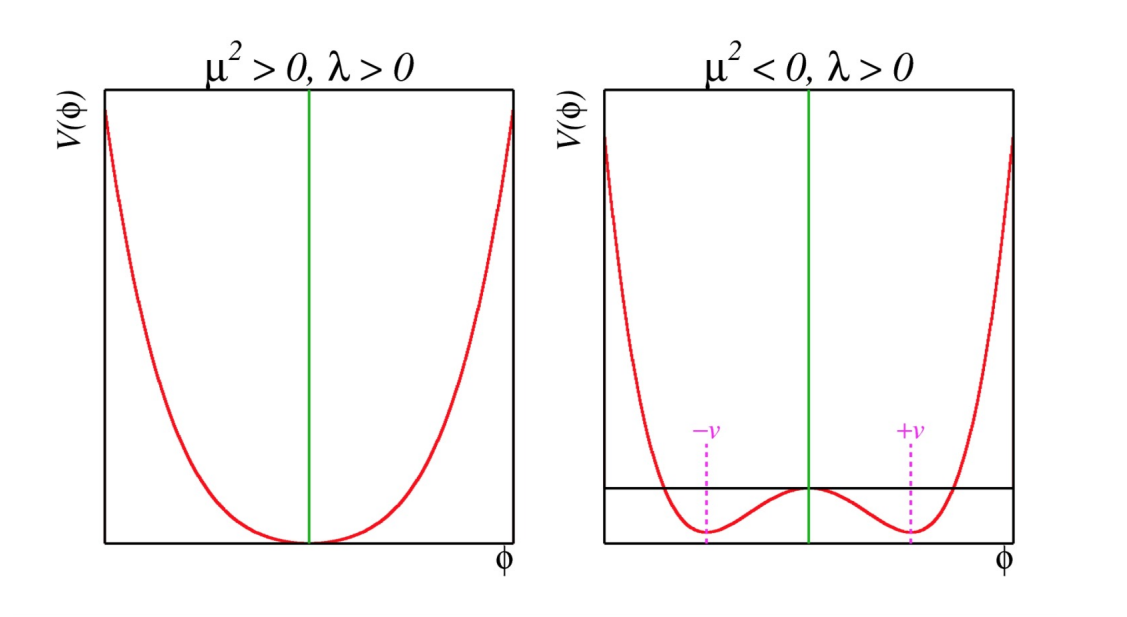
\includegraphics[width=0.7\textwidth]{figures/Theory/Vhiggs.png}
  \caption{Higgs potential $V(\phi)$ with $\mu^{2}>0$ (left) and $\mu^{2}<0$ (right).}
  \label{fig:C2_Higgs_potential}
\end{figure}
Thus, the classical vacuum $\phi_{0}$ of Higgs doublet can be expressed by
\begin{equation}
	\phi_{0} = \frac{1}{\sqrt{2}}\binom{0}{v}
\end{equation}
And to quantize around the classical vacuum in a general form:
\begin{equation}
	\phi = \frac{1}{\sqrt{2}} \binom{0}{v+H}
\end{equation}
Where H is a Hermitian field for physical Higgs scalar.
In this guage, the Lagrangian $L_{Higgs}$ in Eq.~\ref{eq:Lhiggs} takes a simple form
\begin{equation}
\begin{split} \label{eq:Lhiggs2}
	L_{Higgs} & = \left(D^{\mu}\phi\right)^{\dagger}D_{\mu}\phi - V(\phi) \\
	& = M_{W}^{2}W^{\mu+}W_{\mu}^{-}\left(1+\frac{H}{\nu}\right)^{2} + \frac{1}{2}M_{Z}^{2}Z^{\mu}Z_{\mu}\left(1+\frac{H}{\nu}\right)^{2} \\ 
        &   + \frac{1}{2}\left(\partial_{\mu}H\right)^{2} - V(\phi)
\end{split}
\end{equation}
where the W and Z fields are
\begin{equation}
\begin{split}
	& W^{\pm} = \frac{1}{\sqrt{2}} \left(W^{1} \mp iW^{2}\right) \\
	& Z = - sin\theta_{W}B + cos\theta_{W}W^{3}
\end{split}
\end{equation}
Therefore, in Eq.~\ref{eq:Lhiggs2} spontaneous symmetry breaking brings out masses for the W and Z gauge bosons
\begin{equation}
\begin{split}
	& M_{W} = \frac{gv}{2} \\
	& M_{Z} = \sqrt{g^{2} + g'^{2}} \frac{v}{2} = \frac{M_{W}}{cos\theta_{W}}
\end{split}
\end{equation}
where $\theta_{W}$ is the weak angle defined as
\begin{equation}
	sin\theta_{W} = \frac{g'}{\sqrt{g^{2} + g'^{2}}} \qquad cos\theta_{W} = \frac{g}{\sqrt{g^{2} + g'^{2}}} \qquad tan\theta_{W} = \frac{g'}{g}
\end{equation}
Then another gauge boson photon remains massless with the field of
\begin{equation}
	A = cos\theta_{W}B + sin\theta_{W}W^{3}
\end{equation}

After the symmetry breaking, the Higgs potential in unitary gauge can be written into
\begin{equation}
	V(\phi) = -\frac{\mu^{4}}{4\lambda} - \mu^{4}H^{2} + \lambda\nu H^{3} + \frac{\lambda}{4}H^{4}
\end{equation}
The first term in $V$ is a constant, while the second term denotes a (tree-level) mass of Higgs boson
\begin{equation}
	M_{H} = \sqrt{-2\mu^{2}} = \sqrt{2\lambda}v
\end{equation}
Due to the unknown of  quartic Higgs coupling $\lambda$, the Higgs mass is not predicted.
The third and fourth terms in Higgs potential $V$ denote the induced cubic and quartic interactions of the Higgs scalar.

Through the Higgs mechanism, fermions can also acquire their masses.
In the unitary gauge, Yukawa Lagrangian ($L_{Yukawa}$) can be written as a simple form of \cite{Pich:2015lkh}
\begin{equation}
	L_{Yukawa} = -\left(1+\frac{H}{v}\right) \left(m_{d}\bar{d}d + m_{u}\bar{u}u + m_{l}\bar{l}l\right)
\end{equation}
in which $m_{f} = \frac{y_{f}v}{\sqrt{2}}$ for $f = d, u, l$.

%\subsection{Higgs mechanics and electroweak symmetry breaking}
\subsection{Beyond the SM Higgs sector}
\label{bsmhiggs}

After the discovery of the Higgs boson by the ATLAS and CMS Collaborations at the LHC~\cite{20121, 201230} in 2012,
one question comes out: if this Higgs boson at around 125~\gev~ is fully responsible for the unitarization of the scattering amplitudes?
%If not, additional new physics must be present to play this role.
The possibility that this discovered particle is just a part of the extended Higgs sector by various extensions cannot be ruled out.
Many models, motivated by hierarchy and naturalness arguments, 
predicted the extended Higgs sector, such as the electroweak-singlet model and the two-Higgs-doublet models (2HDM).

\textbf{Singlet scalar extension of the SM} \\
The electroweak singlet model can be considered as the minimal extension of the SM Higgs sector~\cite{Profumo_2007}, encompassing a single gauge singlet real scalar field $S$.
In this model, a heavy, real singlet is introduced in addition to the SM one.
The associated zero temperature, tree-level scalar potential can be written as:
\begin{equation}
    V = V_{SM} + V_{HS} + V_{S}
\end{equation}
where
\begin{equation}
\begin{split}
    V_{SM} =  \mu^{2} \left( H^{\dagger}H \right) + \bar{\lambda_{0}} \left( H^{\dagger}H \right) \\
    V_{HS} = \frac{a_{1}}{2}\left( H^{\dagger}H \right)S + \frac{a_{2}}{2}\left( H^{\dagger}H \right)S^{2} \\
    V_{S} = \frac{b_{2}}{2} S^{2} + \frac{b_{3}}{3} S^{3} + \frac{b_{4}}{4} S^{4} \\ 
\end{split}
\end{equation}
where $H$ stands for the SM scalar field of the original Higgs mechanism.
After electroweak symmetry breaking, this model gives rise to two $CP$-even Higgs bosons, in which the lighter one is the Higgs boson that has been discovered at around 125~\gev.
And the new heavy scalar ($S$) is allowed to have both SM and non-SM decays.
One would expect to see suppressions of the branching ratio to SM Higgs decay modes, as the branching ratio to the pair of singlet-like scalars would be considerable. 

\textbf{Two Higgs Doublet Model} \\
The two-Higgs-doublet model (2HDM)~\cite{BRANCO20121} is another extension of SM Higgs sector carried by an additional scalar doublet.
In this model, through electroweak symmetry breaking, there are five physical Higgs bosons: two CP-even, one CP-odd, and two charged ones.
The most general CP-conserving 2HDM has seven free parameters:
\begin{itemize}
    \item The masses of five Higgs bosons: $m_{h}$, $m_{H}$, $m_{A}$ and $m_{H^{\pm}}$.
    \item $tan \beta$: $v_1/v_2$, where $v_1$ and $v_2$ are the two Higgs doublets' vacuum expectation values.
    \item $\alpha$: the two neutral CP-even Higgs bosons mixing angle .
    \item $m_{12}^{2}$: the potential parameter mixing the two Higgs doublets.
\end{itemize}
where the $m_{h}$ can be identified as the mass of observed Higgs boson at around 125~\gev, and $m_{H}$ is another heavy scaler with similar properties to $h$ boson.
The coupling of the neutral Higgs bosons to either $WW$ or $ZZ$ follows the rules~\cite{BRANCO20121}: 
\begin{enumerate}
    \item The coupling of the light Higgs ($h$) equals to the Standard Model coupling times $sin(\beta - \alpha)$ 
    \item The coupling of the heavier Higgs ($H$) equals to the Standard Model coupling times $cos(\alpha - \beta)$.
    \item The coupling of the pseudoscalar ($A$) to vector bosons is zero.
\end{enumerate}
The two Higgs doublets, $\Phi_{1}$ and $\Phi_{2}$, can couple to fermions (leptons and up- and down-type quarks) in several ways, which leads to several types of 2HDM models:
\begin{itemize}
    \item Type-\uppercase\expandafter{\romannumeral1} model: all quarks and leptons couple only to $\Phi_{2}$.
    \item Type-\uppercase\expandafter{\romannumeral2} model: down-type quarks and leptons couple to $\Phi_{1}$, and up-type quarks couple to $\Phi_{2}$.
    \item The ``lepton-specific" model: leptons couple to $\Phi_{1}$, while all quarks couple to $\Phi_{2}$.
    \item The ``flipped" model: down-type quarks couple to $\Phi_{1}$, while up-type quarks and leptons couple to $\Phi_{2}$.
\end{itemize}

%\subsection{Beyond the SM Higgs sector}

\section{Phenomenology of Large Hadron Collider}
The Large Hadron Collider (LHC)~\cite{Bruning:2004ej, Buning:2004wk, Benedikt:2004wm} was built as a bridge between the experiments and the theories.
Physicists hope that the LHC can help to answer some open questions in fundamental physics, 
such as the basic laws of interactions, the forces among the elementary particles, 
the deep structure of space and time, and the interrelation between quantum mechanics and general relativity.
This section will talk about firstly the general introduction of Physics inside hadronic collision,
then followed by two important LHC phenomenologies of the Higgs physics and Diboson physics that are related closely to this dissertation.

\subsection{Physics at hadronic collision}
\label{hadroniccollision}

Protons are not the elementery particle, which actually be composed of quarks and gluons.
So in proton-proton (pp) collision at LHC, it is not protons themselves interact but quarks and gluons.
Scattering processes can then be further classified into either \textit{hard} or \textit{soft} processes
according to the momentum transfer during the interaction \cite{Dremin:2005wd}.
QCD, as an underlying theory for both two process, its approach and level of understandings in two cases are quite different.
For hard process, eg. Higgs, vector bosons and jets production, the rates and event
properties can be precisely predicted based on perturbation theory.
However, for soft processes like total cross-section, the underlying events, the rates and properties are dominated by non-perturbative QCD effects
that are less understood.
For many hard processes, the hard interactions are accompanied by soft ones.
A example of the hadronic collision is illustrated in figure~\ref{fig:C2_had_col}. 
\begin{figure}[!htb]
  \centering
  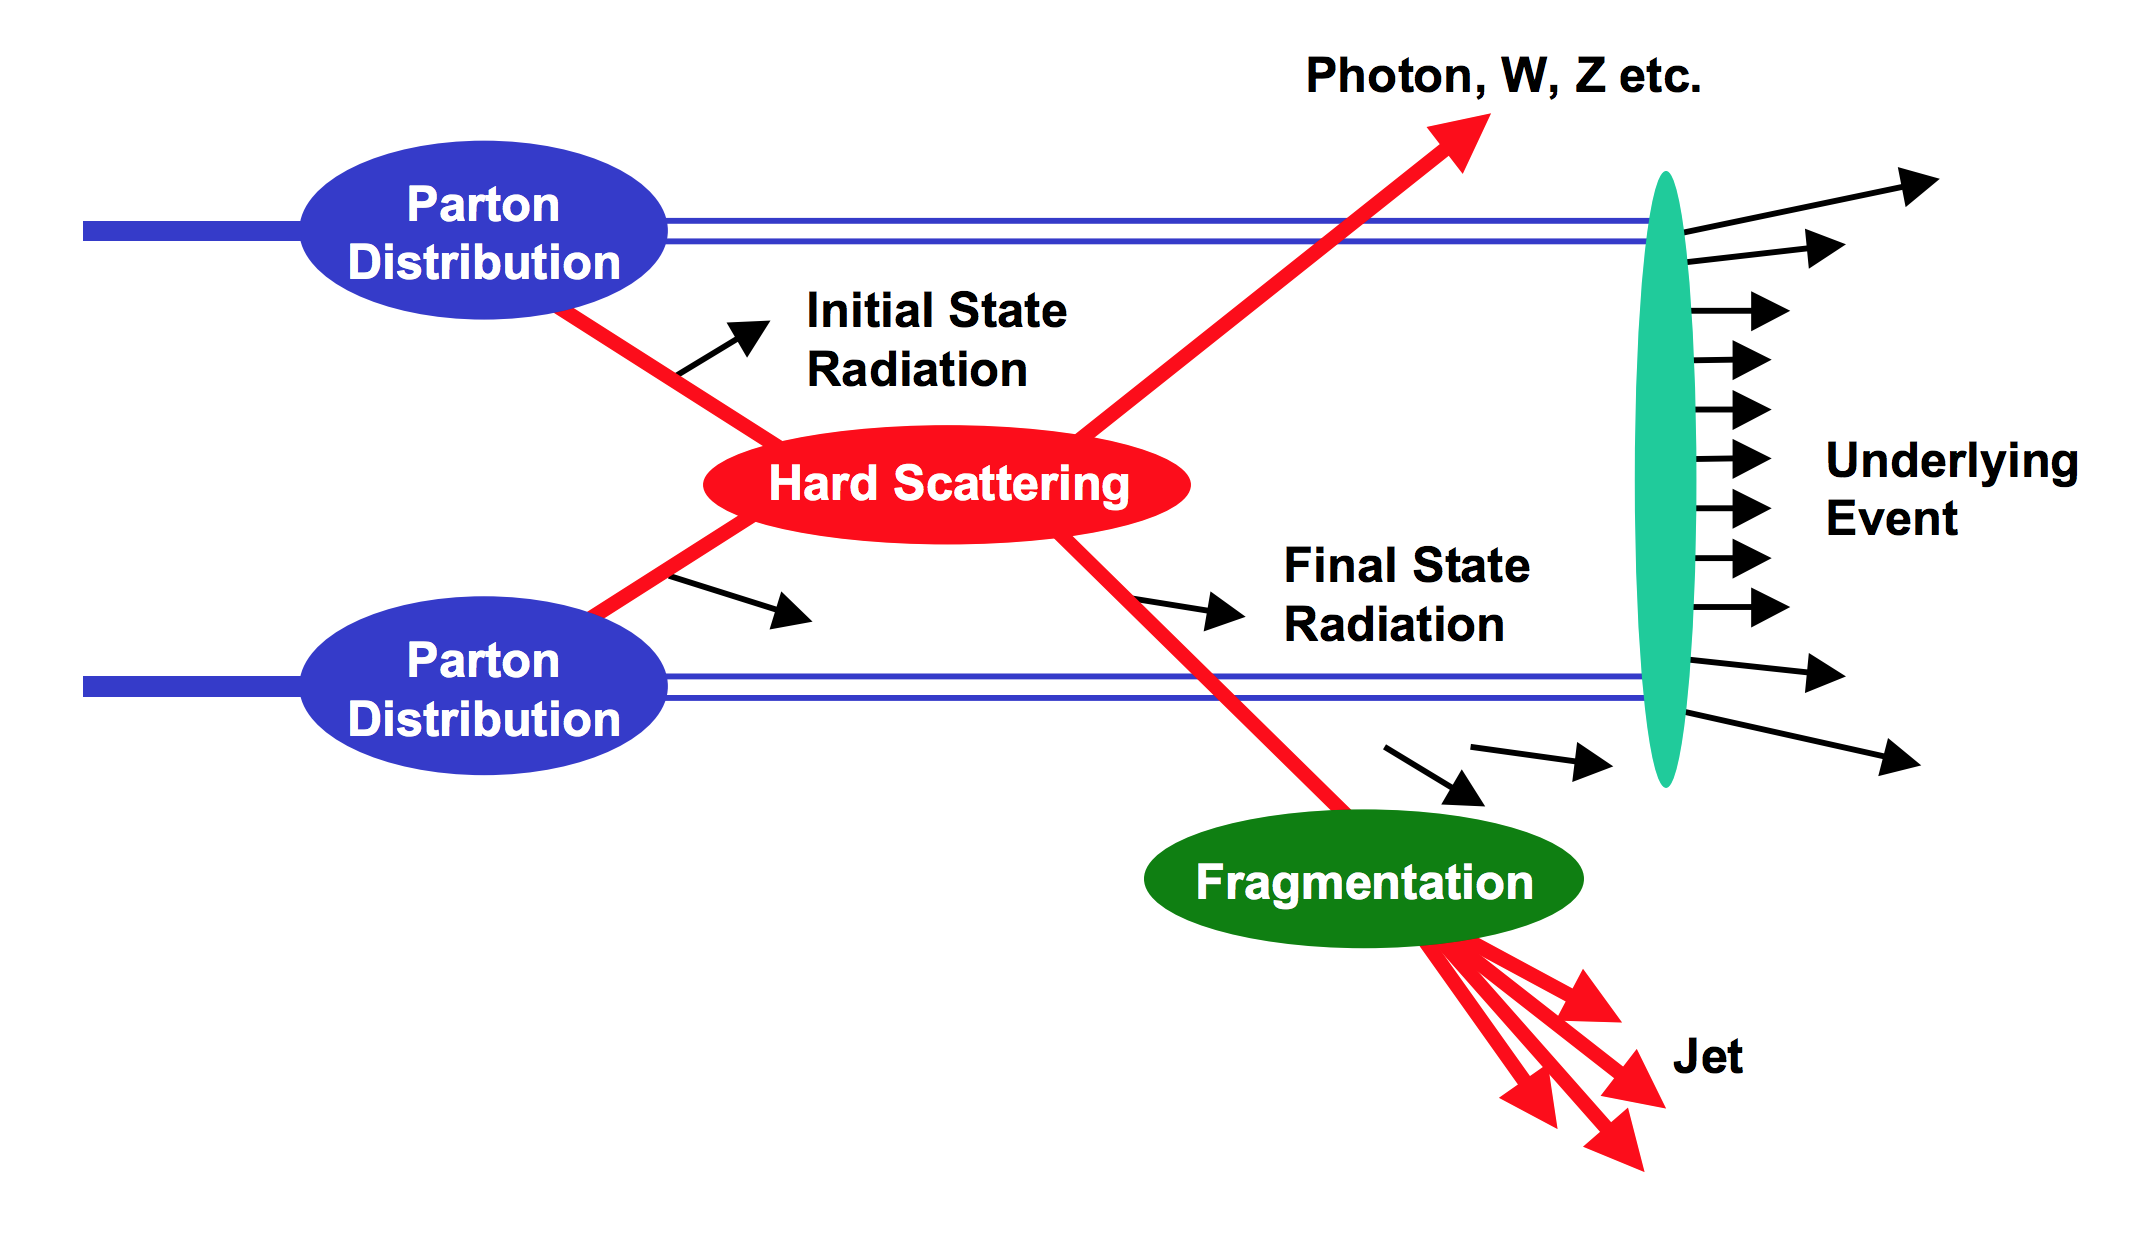
\includegraphics[width=0.7\textwidth]{figures/Theory/hh_collision.png}
  \caption{Schematic view of a hadron-hadron collision \cite{Womersley:2000cx}.}
  \label{fig:C2_had_col}
\end{figure}
and the typical features are summarized as below:
\begin{itemize}
	\item \textbf{Parton Distribution Function (PDF)} $f_{i}\left(x, Q^{2}\right)$ gives the probability of a parton with flavor $i$ (quark or gluon), carring amomentum fraction of $x$ and at the energy of Q in a proton. Parton distribution function cannot be fully calculated by perturbative QCD because of the inherent non-perturbative nature of partons. There are many different sets of PDFs that are determined by a fit to data from experimental observables in various processes. As an example, figure~\ref{fig:C2_PDF4LHC15} for \textit{PDF4LHC15} which is based on the combination of the \textit{CT14}, \textit{MMHT14} and \textit{NNPDF3.1} NNLO PDF sets \cite{Lin:2017snn}.
	\item \textbf{Fragmentation and hadronization} The processes to produce final state particles (or jets) from the partons produced in hard scattering.
	\item \textbf{Initial/Final state radiation} The incoming and outgoing partons that carry color charge can emit QCD radiation, which gives rise to additional jets. Also the charged incoming and outgoing particles can emit QED radiations with photons.
	\item \textbf{Underlying events} Products from soft processes (not come from the primary hard scattering) as the remnants of scattering interactions.
\end{itemize}
\begin{figure}[!htb]
  \centering
  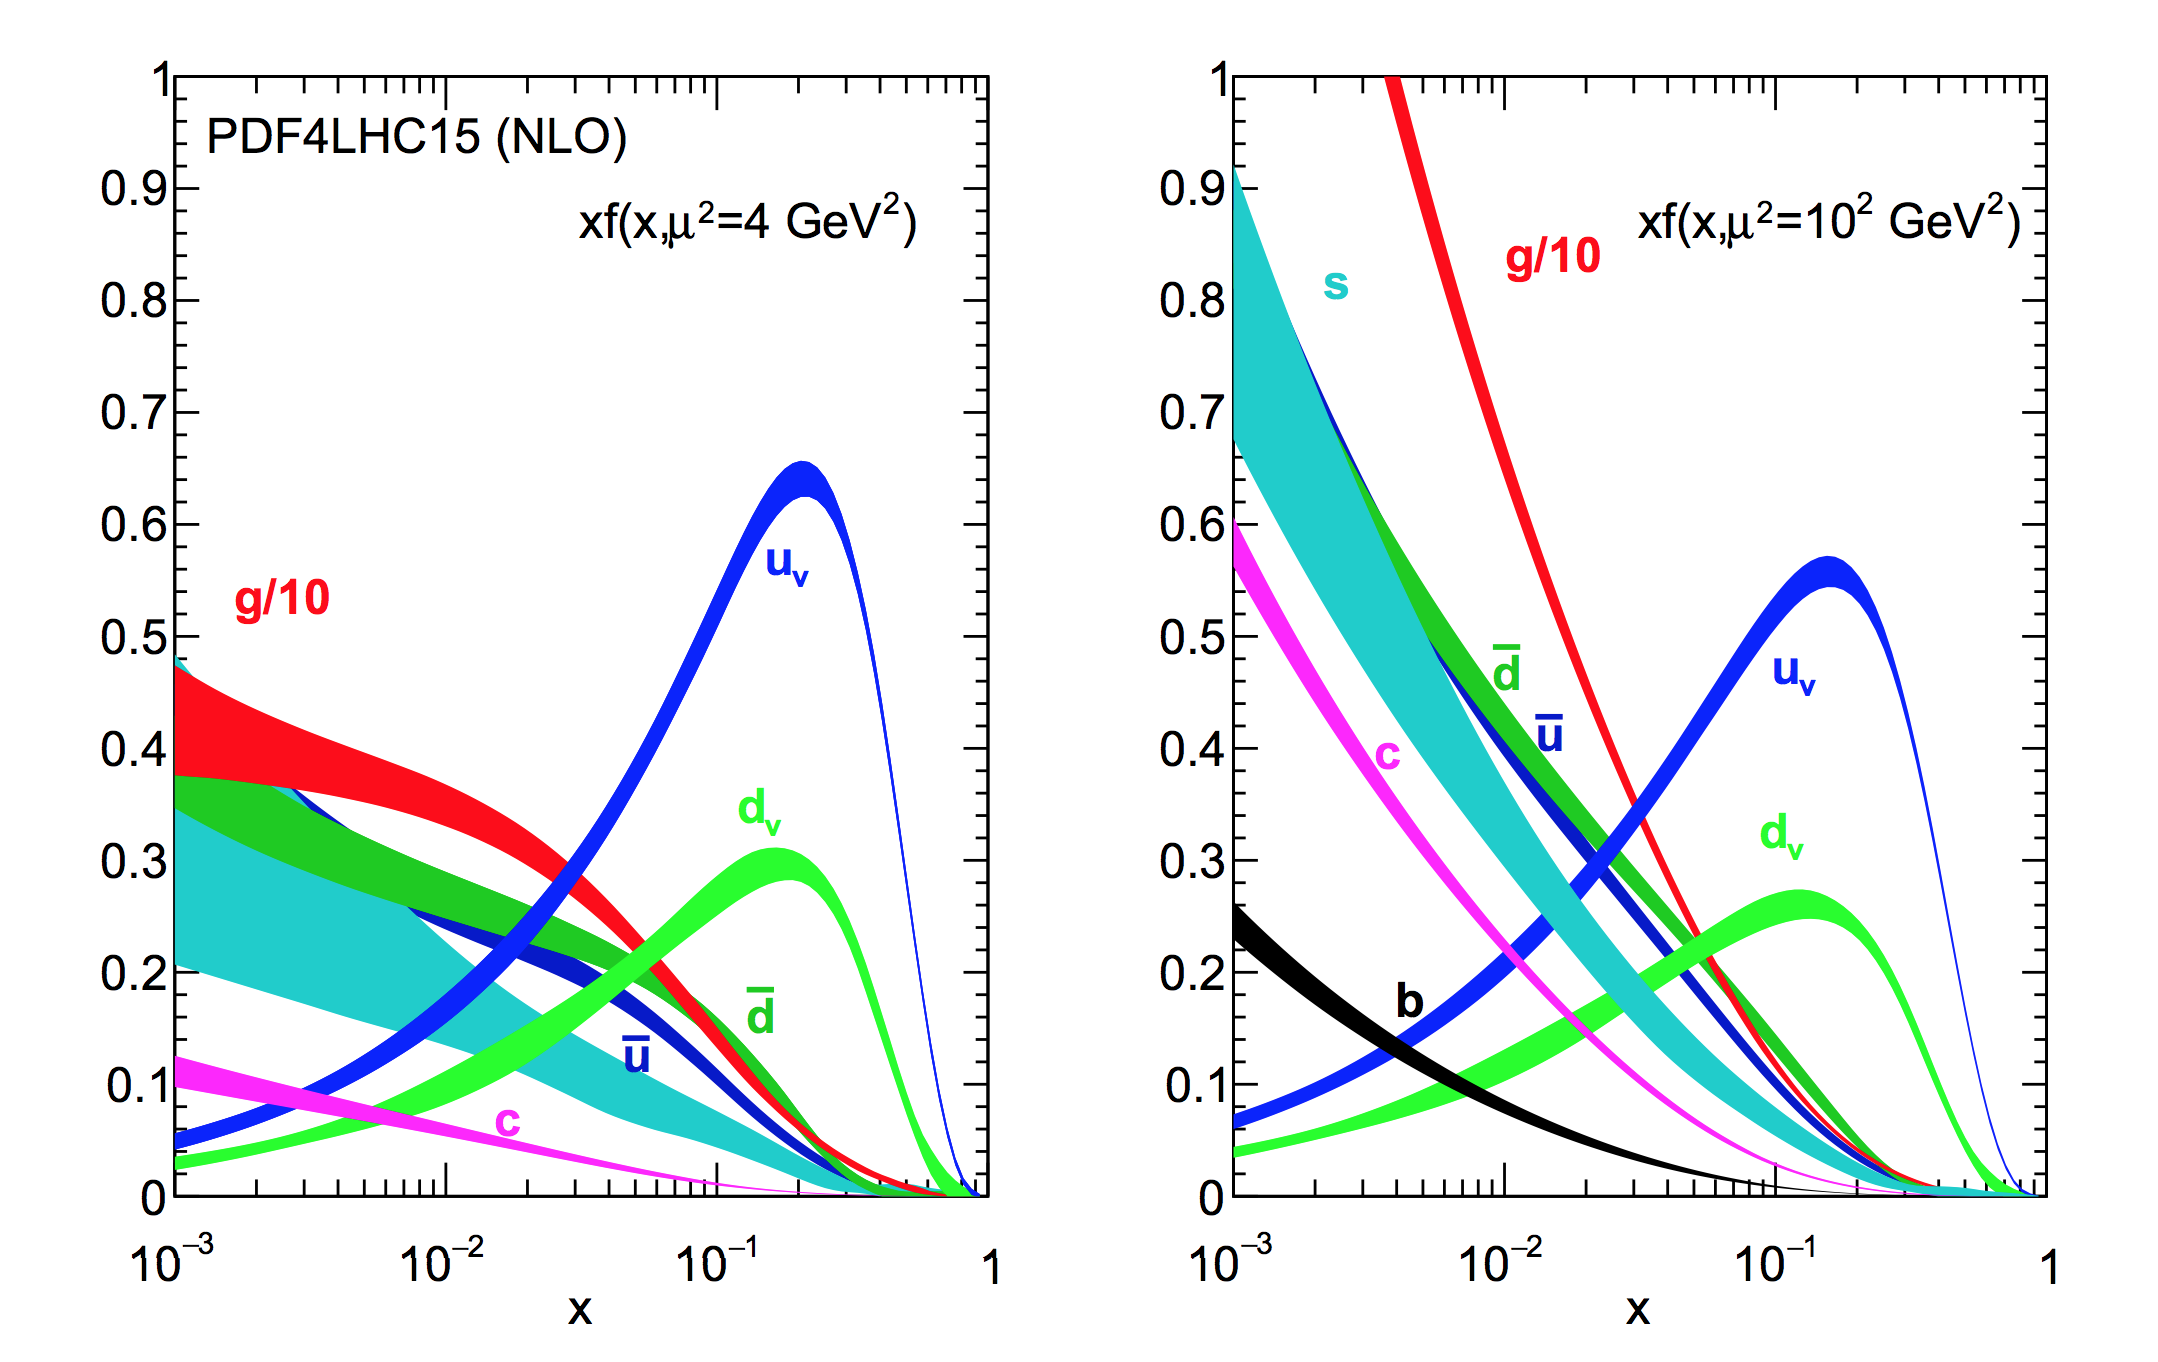
\includegraphics[width=0.7\textwidth]{figures/Theory/PDF4LHC15.png}
  \caption{The PDF4LHC15 NLO PDFs at a low scale $\mu^{2} = Q^{2} = 4 GeV^{2}$ (left) and at $\mu^{2} = Q^{2} = 100 GeV^{2}$ (right) as a function of x.}
  \label{fig:C2_PDF4LHC15}
\end{figure}

\textbf{Cross section of hard scaterring} 

According to \textit{QCD factorization theorems} \cite{Collins:1989gx}, the perturbative calculations can be applied to many important
hard processes involving hadrons. The basic problem addressed by factorization theorems is how to calculate high energy cross sections.
Conder the process of scattering between two hardons A and B to produce a final state X, the cross section $\sigma$ can be obtained 
by summing over all the subprocess cross section $\hat{\sigma}$ \cite{Stirling:1194745}
\begin{equation}
	\sigma_{AB} = \int dx_{a} dx_{b} f_{a/A}\left(x_{a}\right) f_{b/B}\left(x_{b}\right) \hat{\sigma}_{ab\rightarrow X}
\end{equation}
where $f_{q/A}\left(x_{q}\right)$ is the parton distrition functions of parton $q$.
Taking into account the leading order correction:
\begin{equation} \label{eq:xs2}
	\sigma_{AB} = \int dx_{a} dx_{b} f_{a/A}\left(x_{a}Q^{2}\right) f_{b/B}\left(x_{b}Q^{2}\right) \hat{\sigma}_{ab\rightarrow X}
\end{equation}
where $Q^{2}$ represents large momentum scale that characterizes the hard scattering.
Later on, since the finite corrections were not universal and had to be calculated separately for each process,
the perturbative $O\left(\alpha_{S}^{n}\right)$ corrections to the leading logarithm cross section in Eq.~\ref{eq:xs2}
need to be applied, one can get:
\begin{equation}
	\sigma_{AB} = \int dx_{a} dx_{b} f_{a/A}\left(x_{a}\mu_{F}^{2}\right) f_{b/B}\left(x_{b}\mu_{F}^{2}\right) \hat{\sigma}_{ab\rightarrow X}\left(\alpha_{S},\mu_{R},\mu_{F}\right)
\end{equation}
in which $\mu_{F}$ is \textit{factorization scale} which can represent the scale that separates the long- and short-distance physics,
and $\mu_{R}$ is the \textit{renormalization scale} for QCD running coupling.
$\hat{\sigma}_{ab\rightarrow X}$ is the parton-level hard scattering cross section that can be calculated perturbatively in QCD with the form of
\begin{equation} \label{eq:xs3}
	\hat{\sigma}_{ab\rightarrow X}\left(\alpha_{S},\mu_{R},\mu_{F}\right) 
		= \left(\alpha_{S}\right)^{n} \left[ \hat{\sigma}^{(0)}
		+ \left(\alpha_{S}/2\pi\right) \hat{\sigma}^{(1)}\left(\mu_{R},\mu_{F}\right)
		+ \left(\alpha_{S}/2\pi\right)^{2} \hat{\sigma}^{(2)}\left(\mu_{R},\mu_{F}\right)
		+ ... \right]
\end{equation}
where $\hat{\sigma}^{(0)}$ stands for the leading-order (LO) partonic cross section,
while $\hat{\sigma}^{(1)}$ and $\hat{\sigma}^{(2)}$ are the next-to-leading-order (NLO) and
next-to-next-to-leading-order (NNLO) cross section.

$\mu_{R}$ and $\mu_{F}$ depend on the order of truncation in Eq.~\ref{eq:xs3}.
In principle, if cross section is calculated to all orders, it is invariant under changes in these parameters.
The choices of $\mu_{R}$ and $\mu_{F}$ are arbitrary. 
To avoid unnaturally large logarithms reappearing in the perturbation series,
it is sensible to choose $\mu_{R}$ and $\mu_{F}$ values of the order of the typical momentum scales of
the hard scattering process and $\mu_{R} = \mu_{F}$ is also often assumed.
Take Drell–Yan process as an example, the standard choice is $\mu_{R} = \mu_{F} = m_{ll}$, 
where $m_{ll}$ is the invariant mass of dilepton pair.

%\subsection{Physics at hadron colliders}
\subsection{Higgs physics at LHC}
\label{higgs}

One important physics purpose of LHC is searching for Higgs boson, which was the last missing part in SM.
This section will talk about both the production and decay modes of SM Higgs boson in proton-proton collision.

%% ================================ Higgs production ===============================
\textbf{Higgs productions}

Higgs boson can be produced through several processes.
There are 4 main production modes at LHC: gluon-gluon fusion (\textit{ggF}), vector boson fusion (\textit{VBF}),
associated production with vector-bosons (also called Higgs strahlung) (\textit{VH}) 
and associated production with a pair of top/antitop quarks (\textit{ttH}) \cite{Grojean:2243593}.
Figure~\ref{fig:higgs_productions_fd} shows the corresponding Feynman diagrams of each process (at LO).
\begin{figure}[!htb]
  \centering
  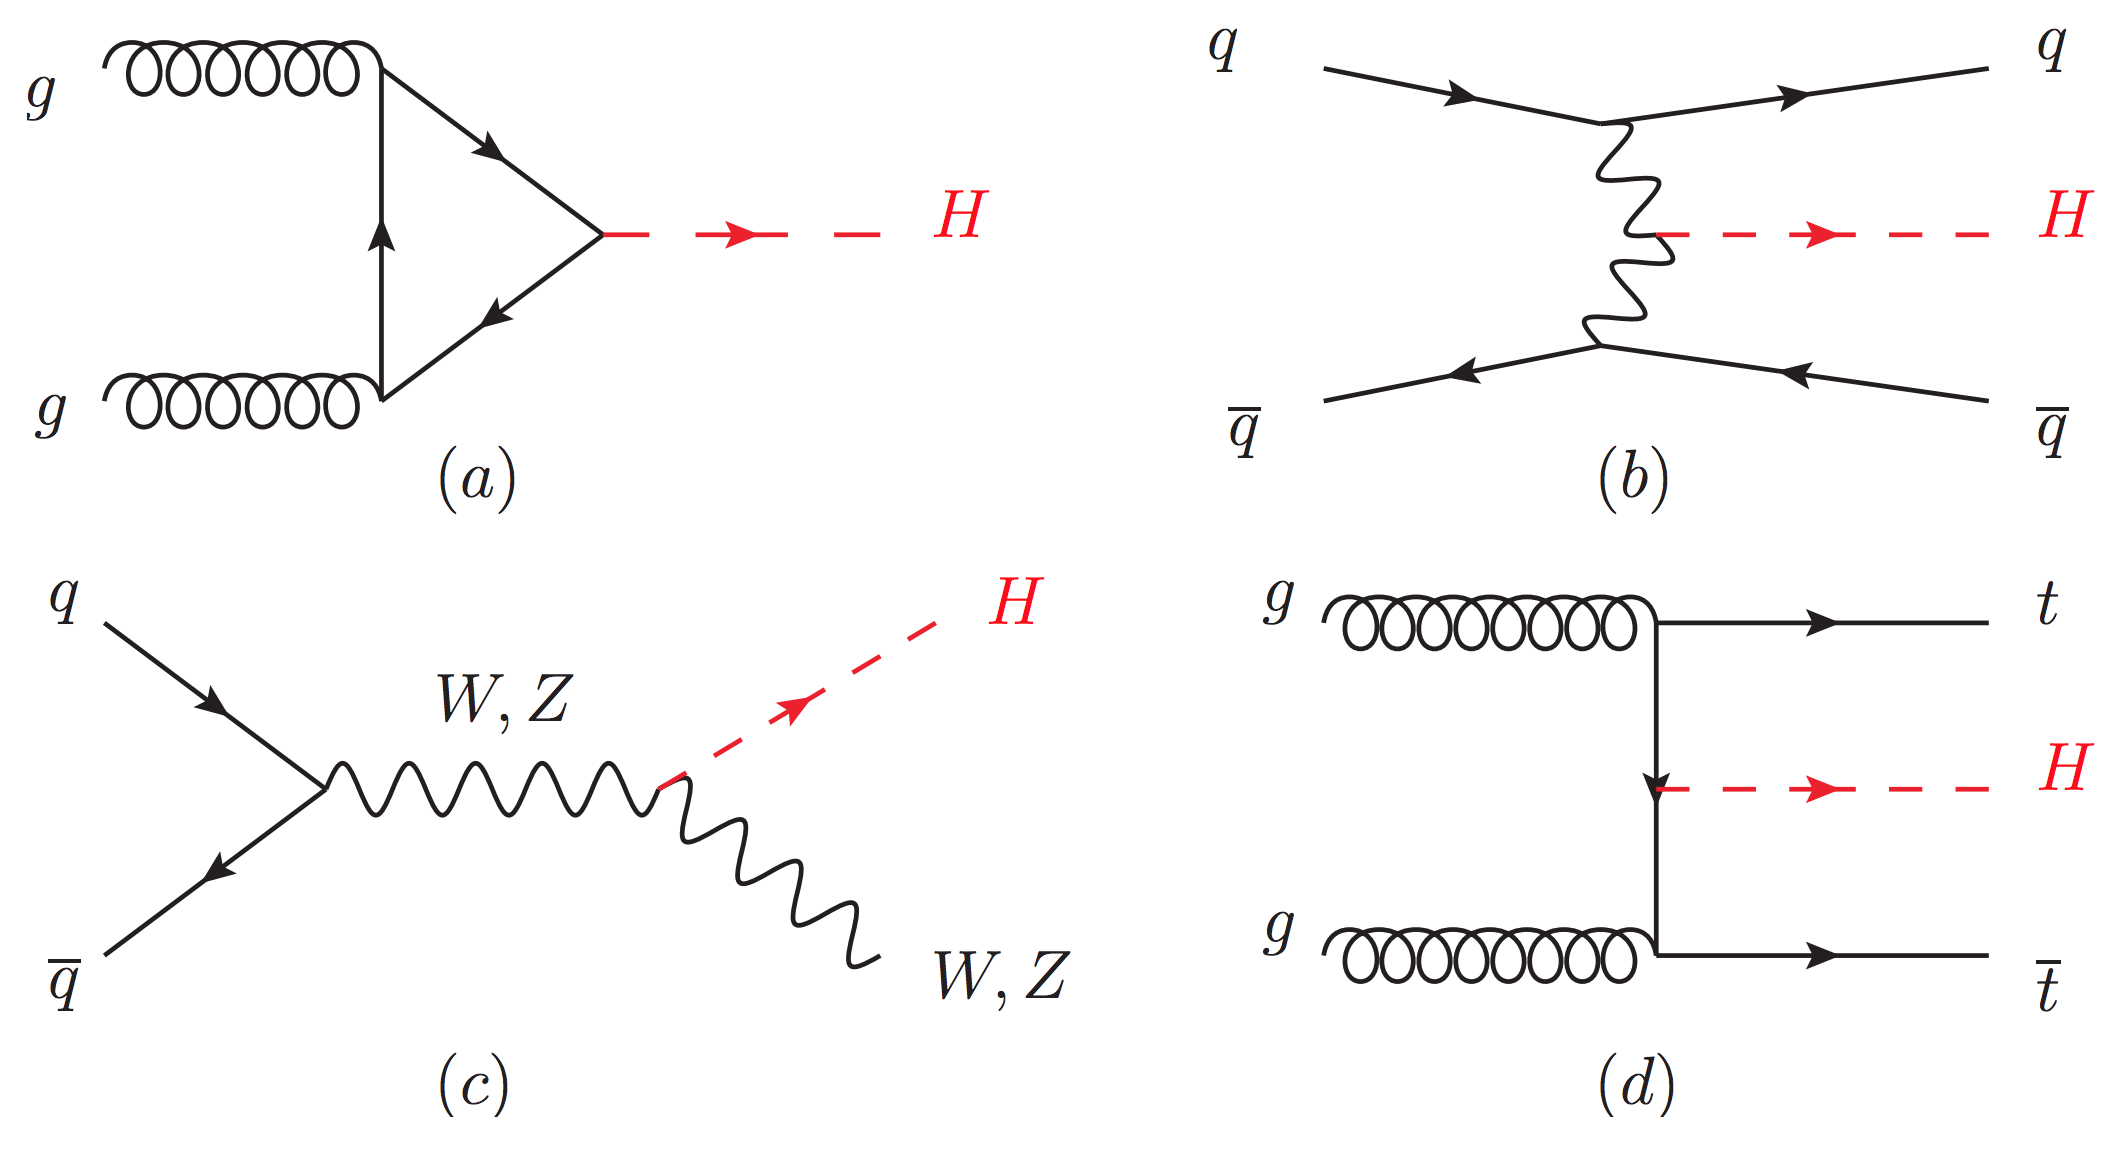
\includegraphics[width=0.8\textwidth]{figures/Theory/Figures_FeynmanHprod.png}
  \caption{Feynman diagrams of the Higgs production modes:
	   (a) ggF; (b) VBF; (c) VH; (d) ttH.}
  \label{fig:higgs_productions_fd}
\end{figure}
For pp collision, the cross section of productions of Higgs boson is as a function of center-of-mass-energy $\sqrt{s}$. 
Figure~\ref{fig:higgs_productions_xs} summarizes the cross section for SM Higgs with mass of 125 GeV.\\
\begin{figure}[!htb]
  \centering
  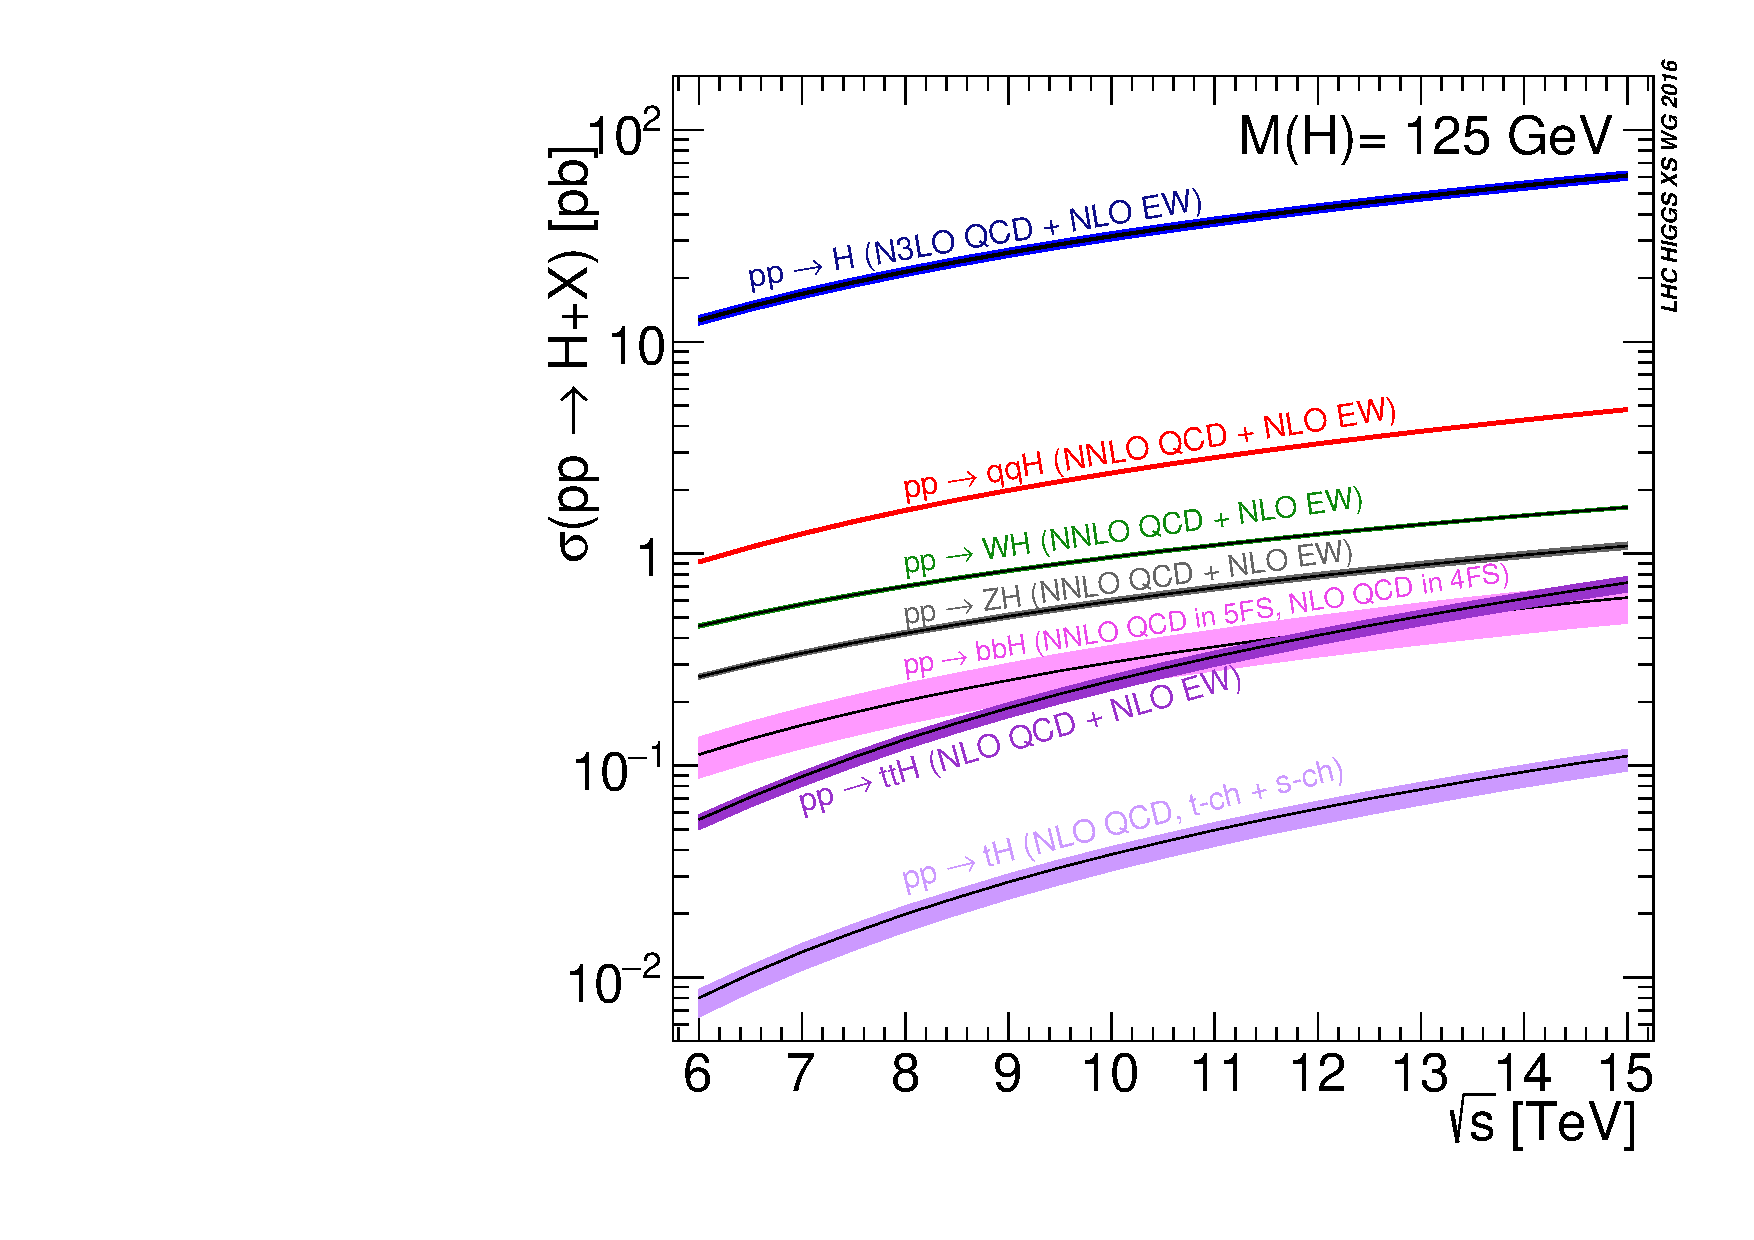
\includegraphics[width=0.5\textwidth]{figures/Theory/Plot_Escan_H125_new_sqrt.pdf}
  \caption{The SM Higgs boson production cross sections as a function of the center-of-mass-energy for pp collision.}
  \label{fig:higgs_productions_xs}
\end{figure}
Figure~\ref{fig:higgs_productions_xs2} summarizes the prospect of different Higgs boson production cross sections 
as a function of Higgs mass for pp collision center-of-mass-energy at 13 TeV and 14 TeV \cite{deFlorian:2227475}. 
\begin{figure}[!htb]
  \centering
  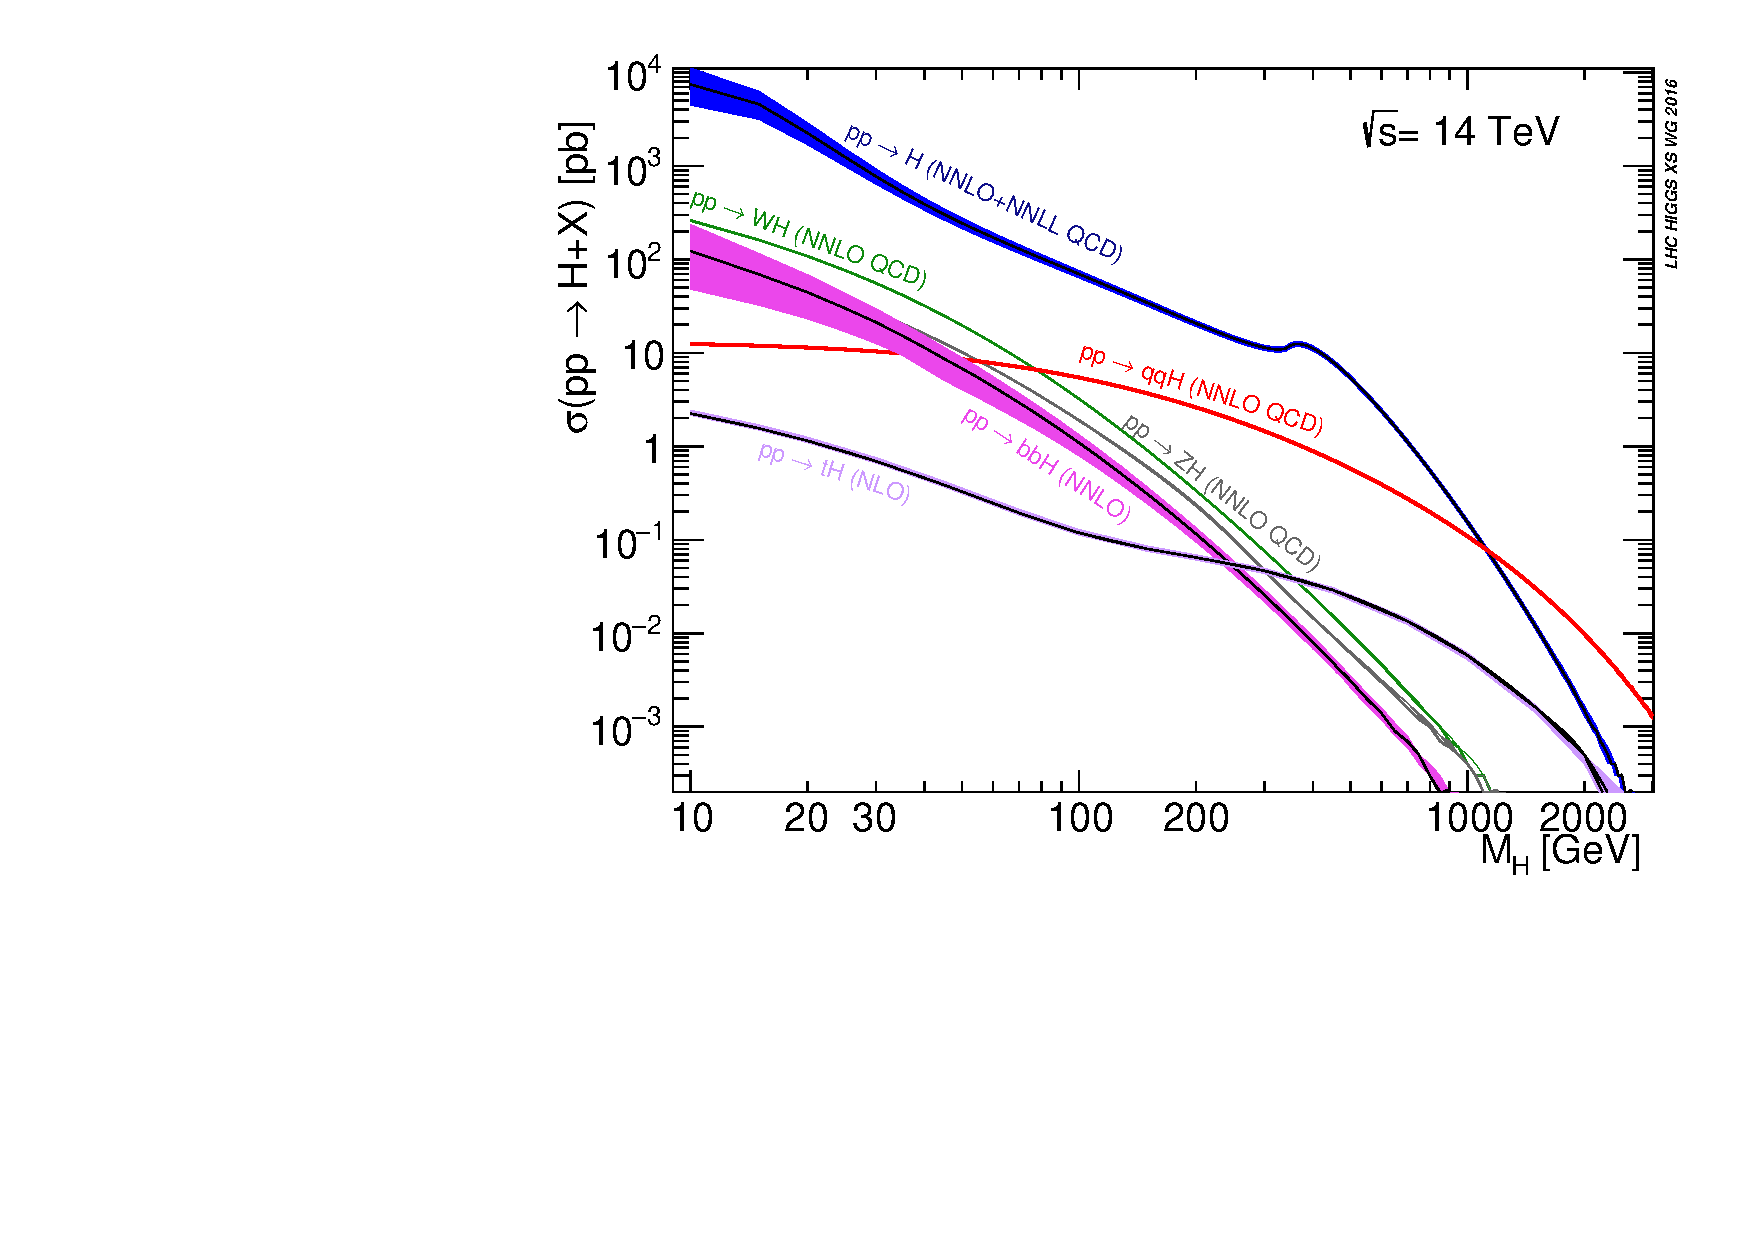
\includegraphics[width=0.45\textwidth]{figures/Theory/plotAll_14tev_BSM_sqrt.pdf}
  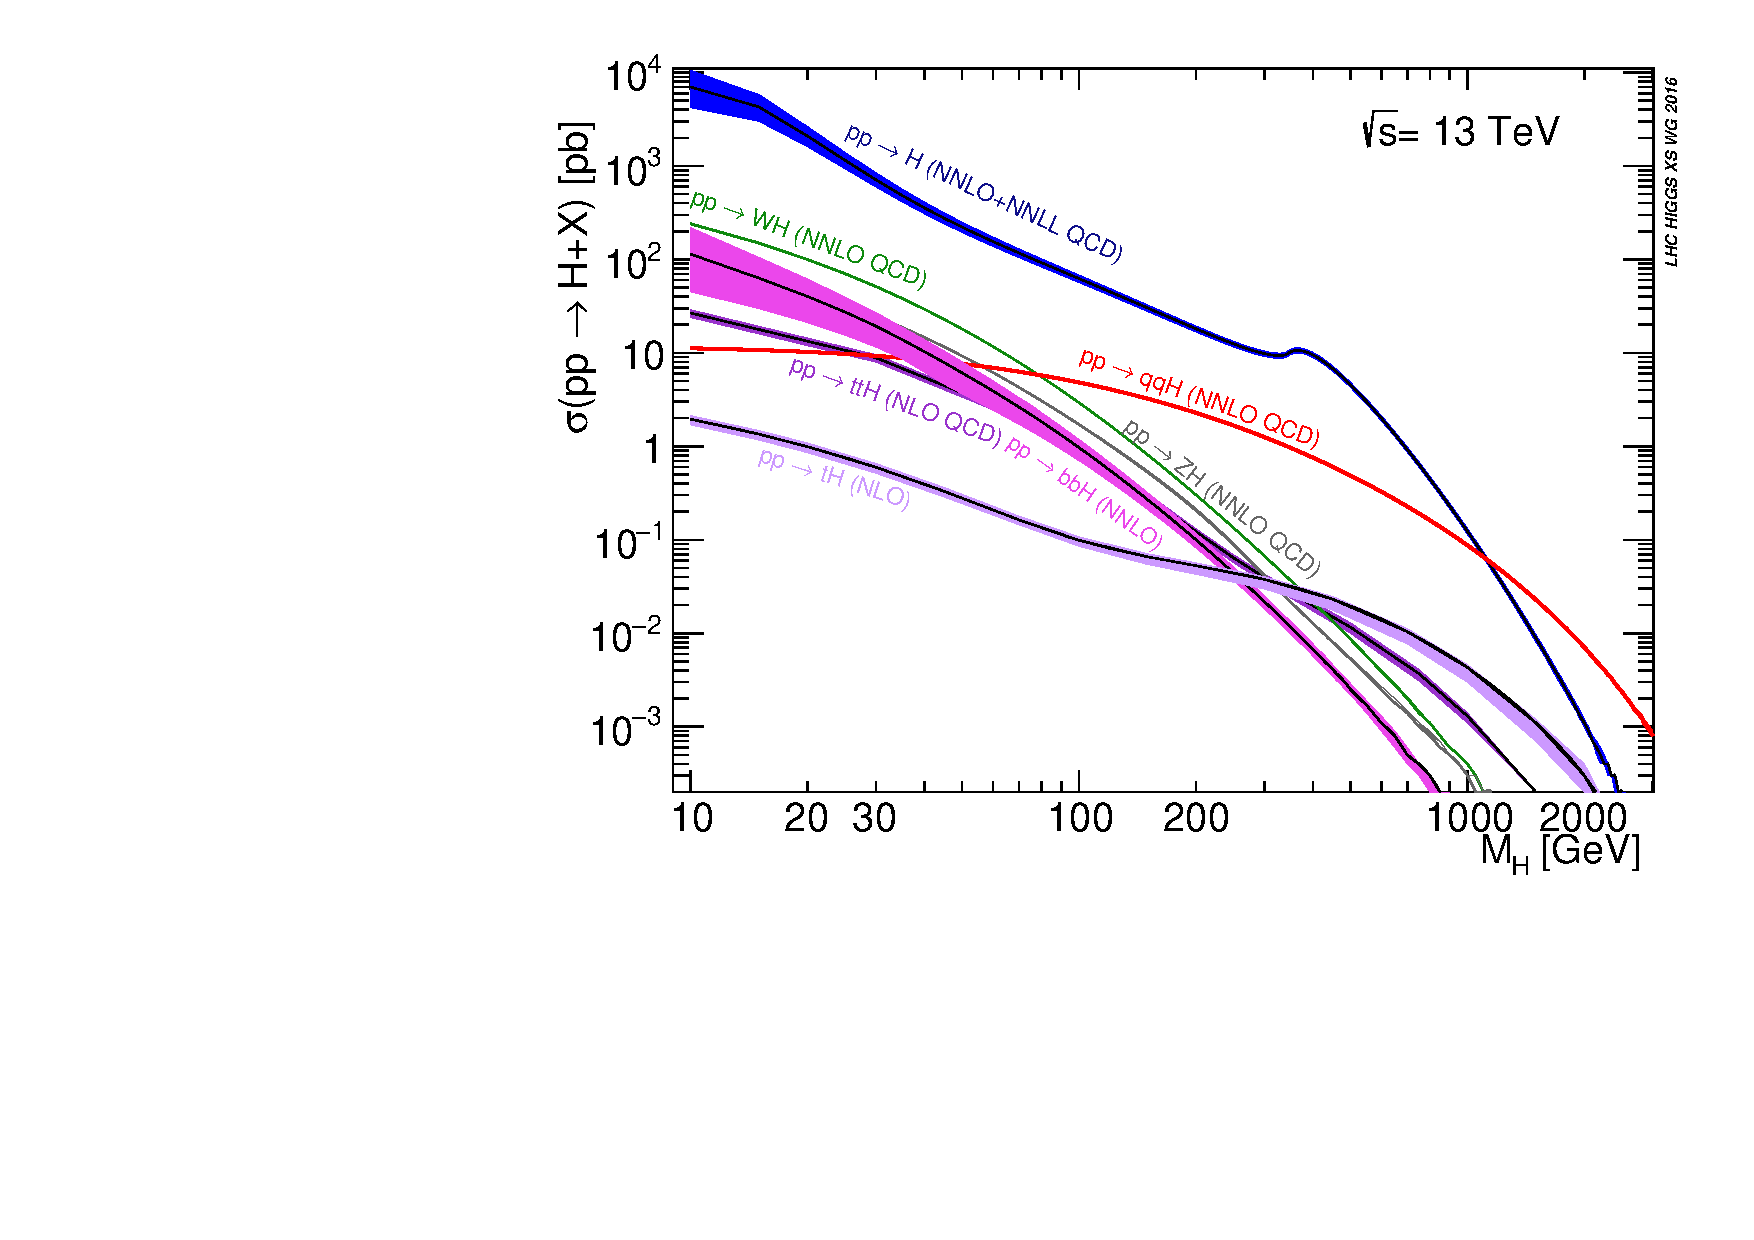
\includegraphics[width=0.45\textwidth]{figures/Theory/plotAll_13tev_BSM_sqrt.pdf}
  \caption{Higgs boson production cross section for various production modes as a function of the Higgs mass mH for $\sqrt{s}$ = 13 TeV (left) and 14 TeV (right) for pp collision.}
  \label{fig:higgs_productions_xs2}
\end{figure}

%% ================================ Higgs decays ===================================
\textbf{Higgs decays}

Higgs boson can interact with gauge bosons and fermions through gauge coupling and Yukawa coupling as introduced in section~\ref{symbreaking}.
Figure~\ref{fig:higgs_decay_fd} depicts Feynman diagrams of possible Higgs decay channels.
\begin{figure}[!htb]
  \centering
  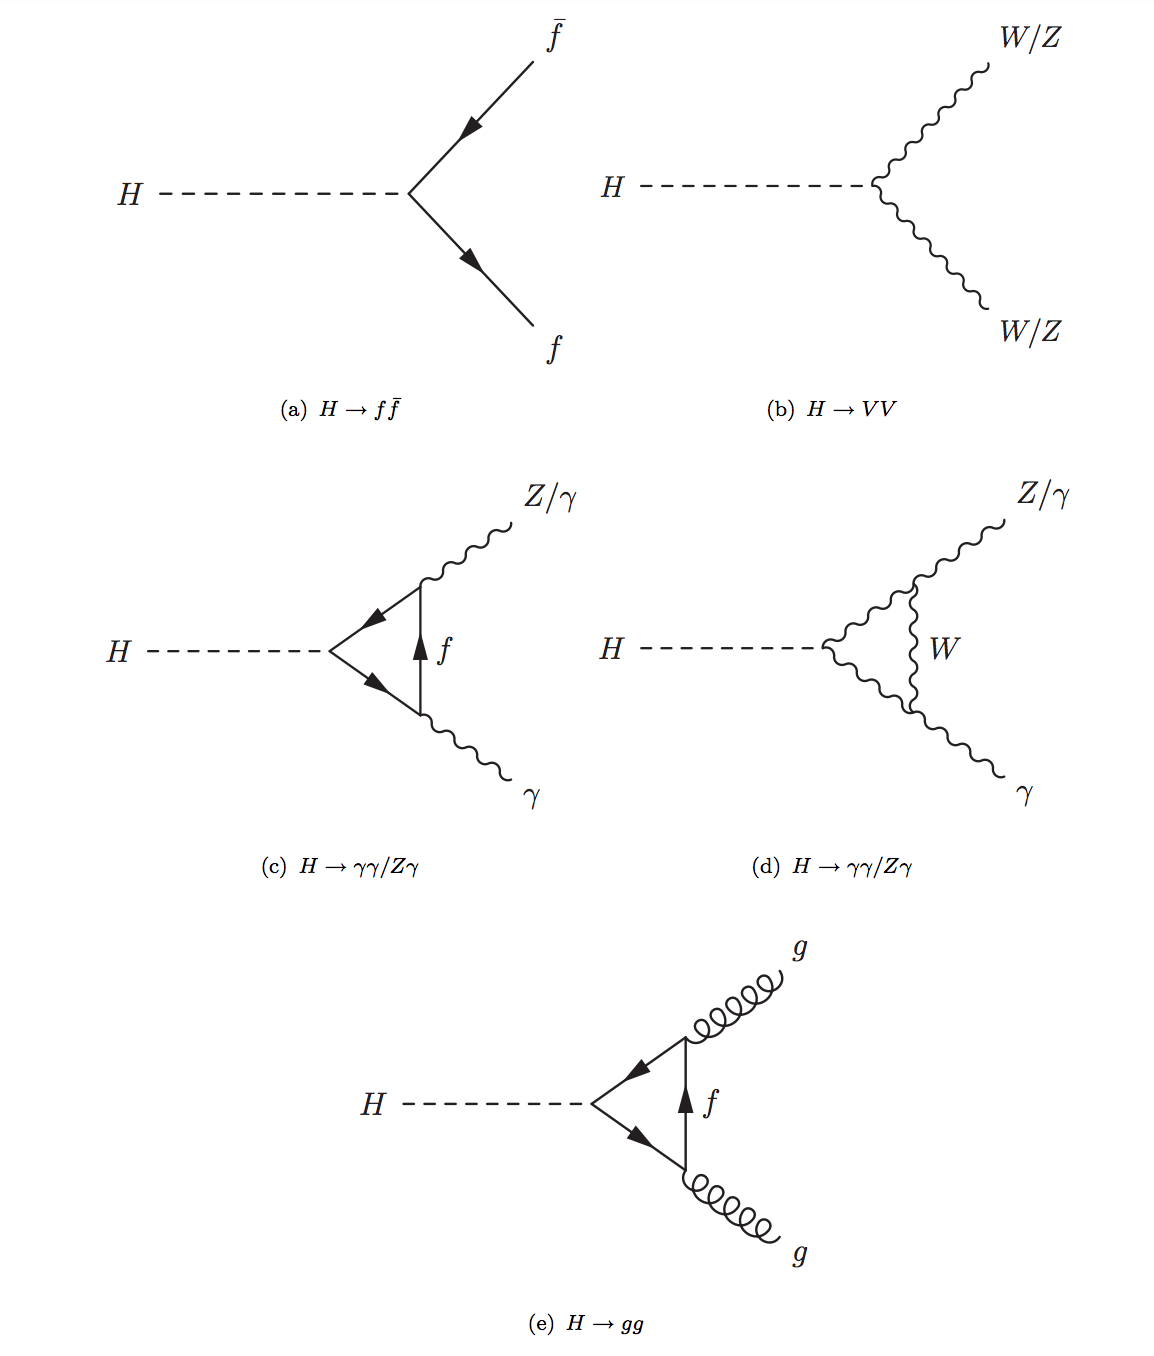
\includegraphics[width=0.8\textwidth]{figures/Theory/Figures_Feynman_Hdecay.png}
  \caption{SM Higgs decay channels.}
  \label{fig:higgs_decay_fd}
\end{figure}
The branching ratio of Higgs boson decaying into different final states as a function of Higgs mass is shown in figure~\ref{fig:higgs_decay_br}.
\begin{figure}[!htb]
  \centering
  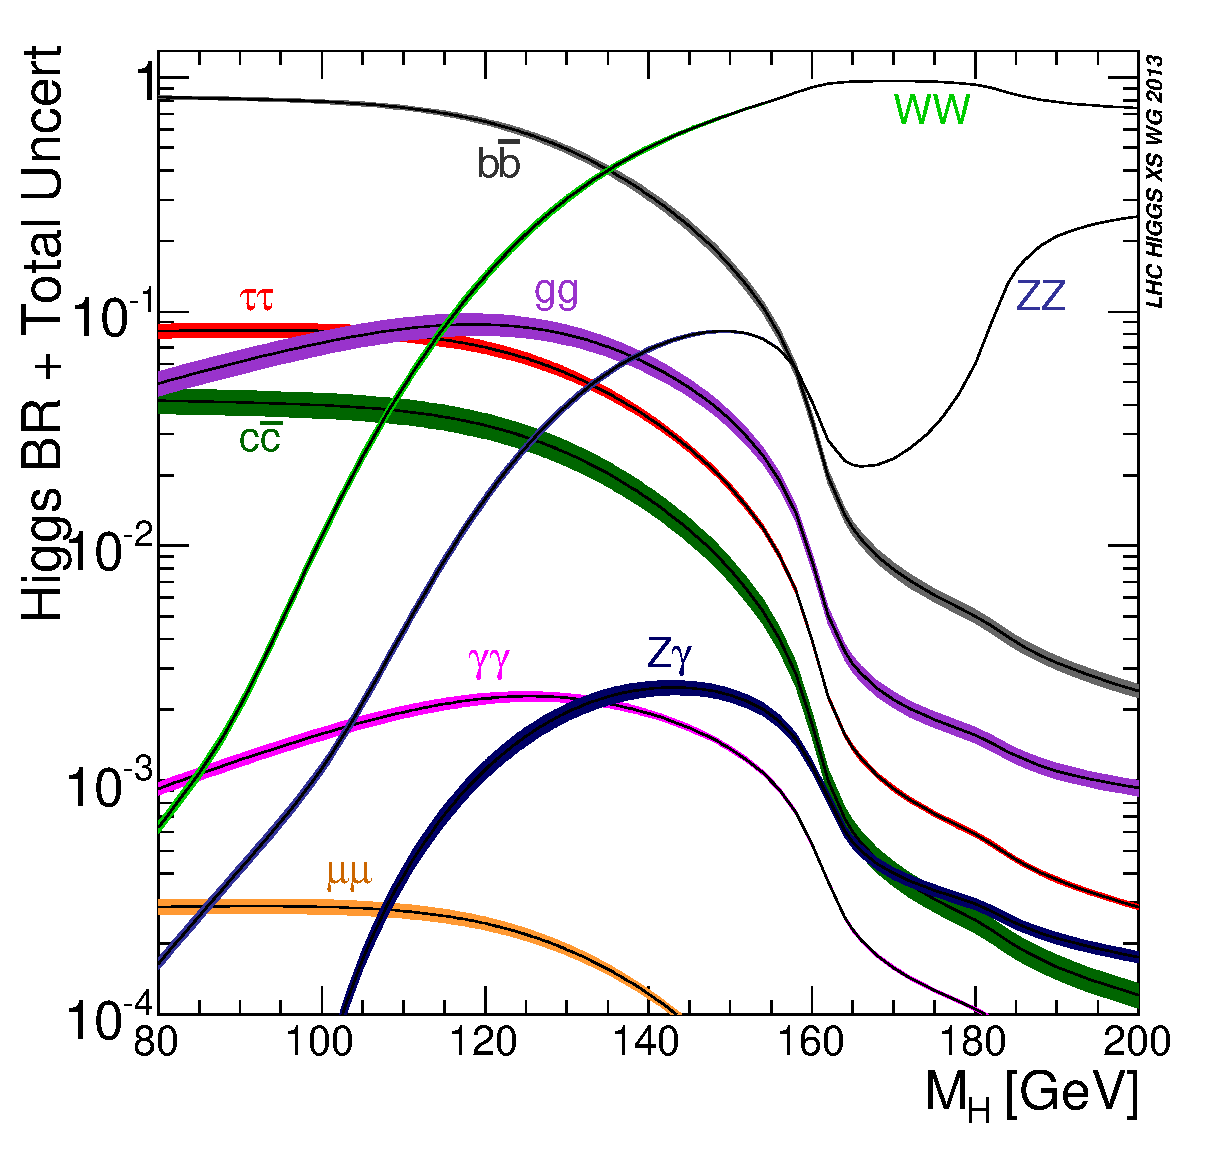
\includegraphics[width=0.5\textwidth]{figures/Theory/Higgs_BR_LM.eps}
  \caption{Branching ratio of Higgs decays \cite{Heinemeyer:1559921}. }
  \label{fig:higgs_decay_br}
\end{figure} 

%% ====================================== High mass related ===========================
(\textbf{BSM Higgs models})



%\subsection{Higgs Physics at LHC}
\subsection{Diboson physics}
\label{diboson}

The study of diboson physics is another important test for SM of particle physics in electroweak sector, 
in which vector boson scattering is a key process for probing the mechanism of electroweak symmetry breaking (EWSB).
In the meantime, the non-resonant diboson productions are crucial backgrounds for Higgs study at LHC, which make the precise measurement of their cross section becomes very important.

%% ====================================== Diboson productions ========================
\textbf{Diboson productions}

About $90\%$ of diboson productions at hadron collider is from quark-antiquark annihilation,
while others are contributed from gluon initiated process.
Figure~\ref{fig:diboson_fd1} shows the tree-level Feynman diagrams of diboson production.
\begin{figure}[!htb]
  \centering
  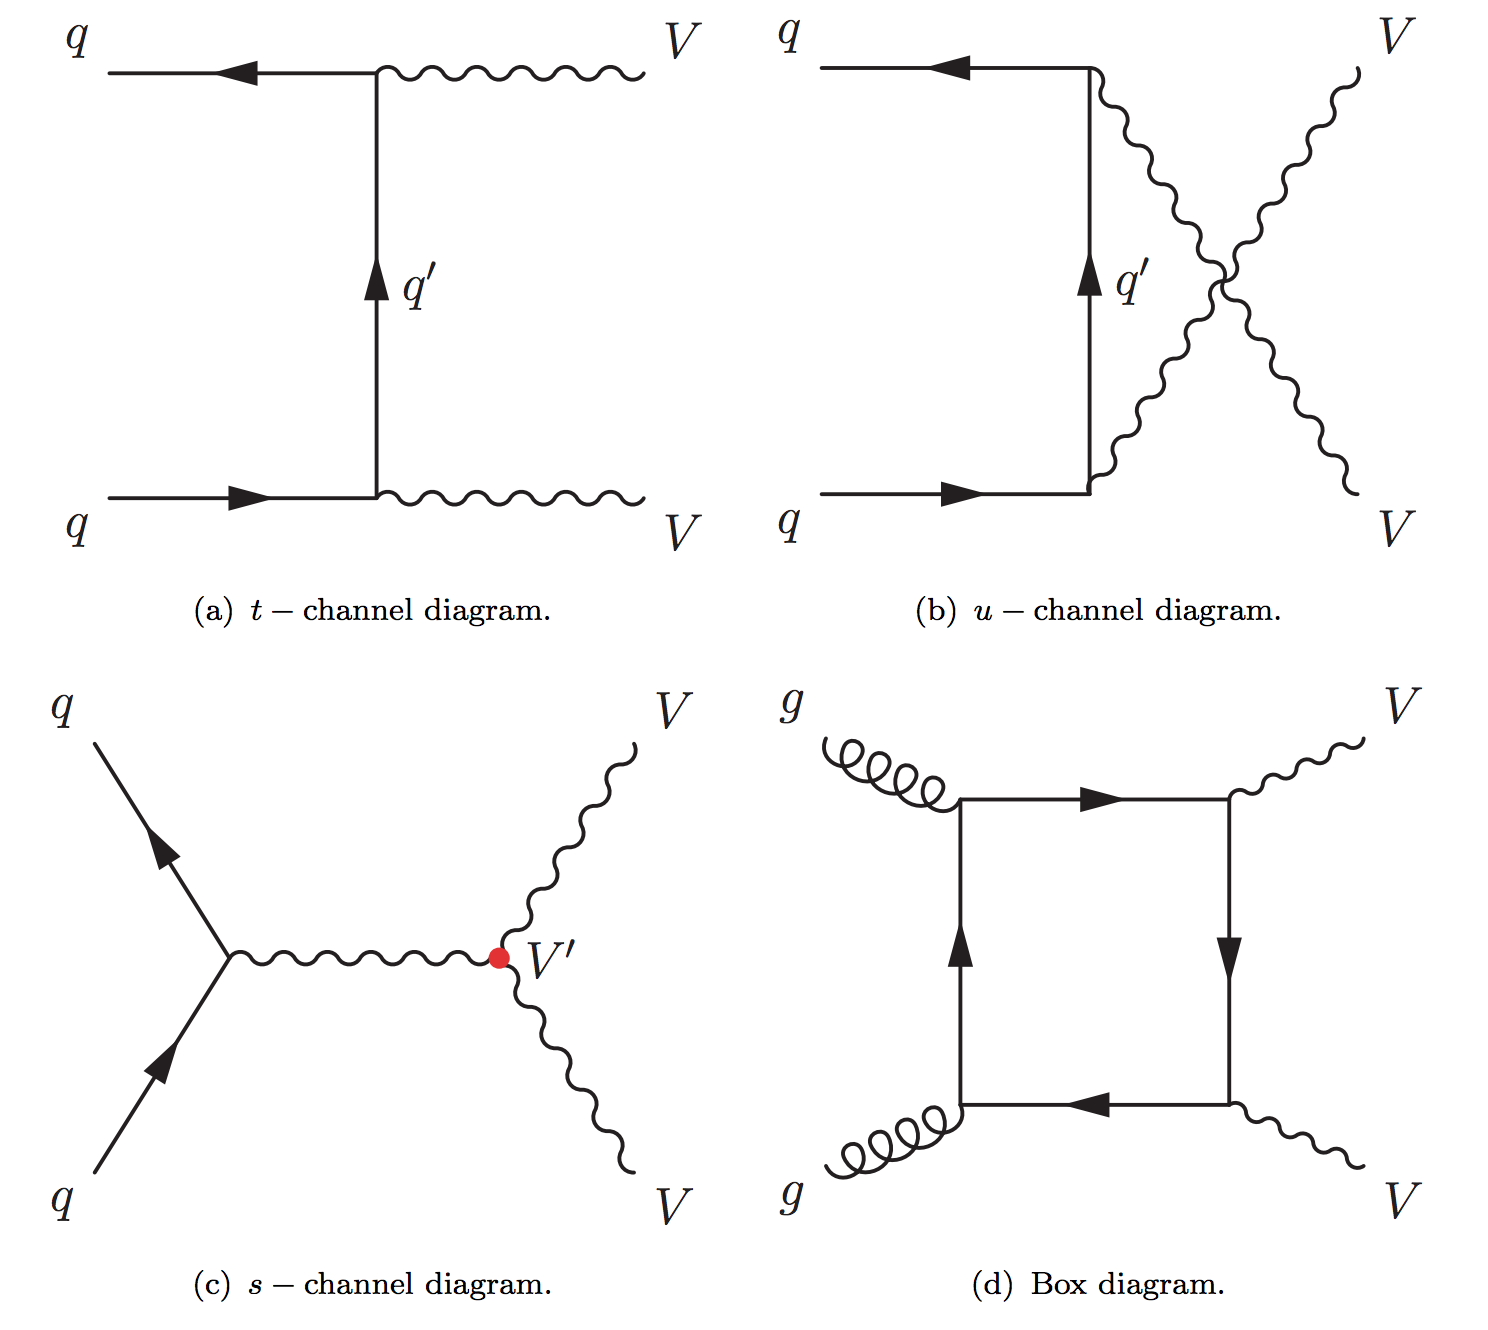
\includegraphics[width=0.7\textwidth]{figures/Theory/diboson_prod_fey.png}
  \caption{The tree-level Feynman diagrams of diboson production at LHC.}
  \label{fig:diboson_fd1}
\end{figure}
Then figure~\ref{fig:diboson_xs1} illuminates the total production cross-section presented by ATLAS
as a function of centre-of-mass energy $\sqrt{s}$ from 7 to 13 TeV for several diboson processes comparing 
to some other major processes in hardon collision.
The cross section for diboson processes are measured at NNLO. 
\begin{figure}[!htb]
  \centering
  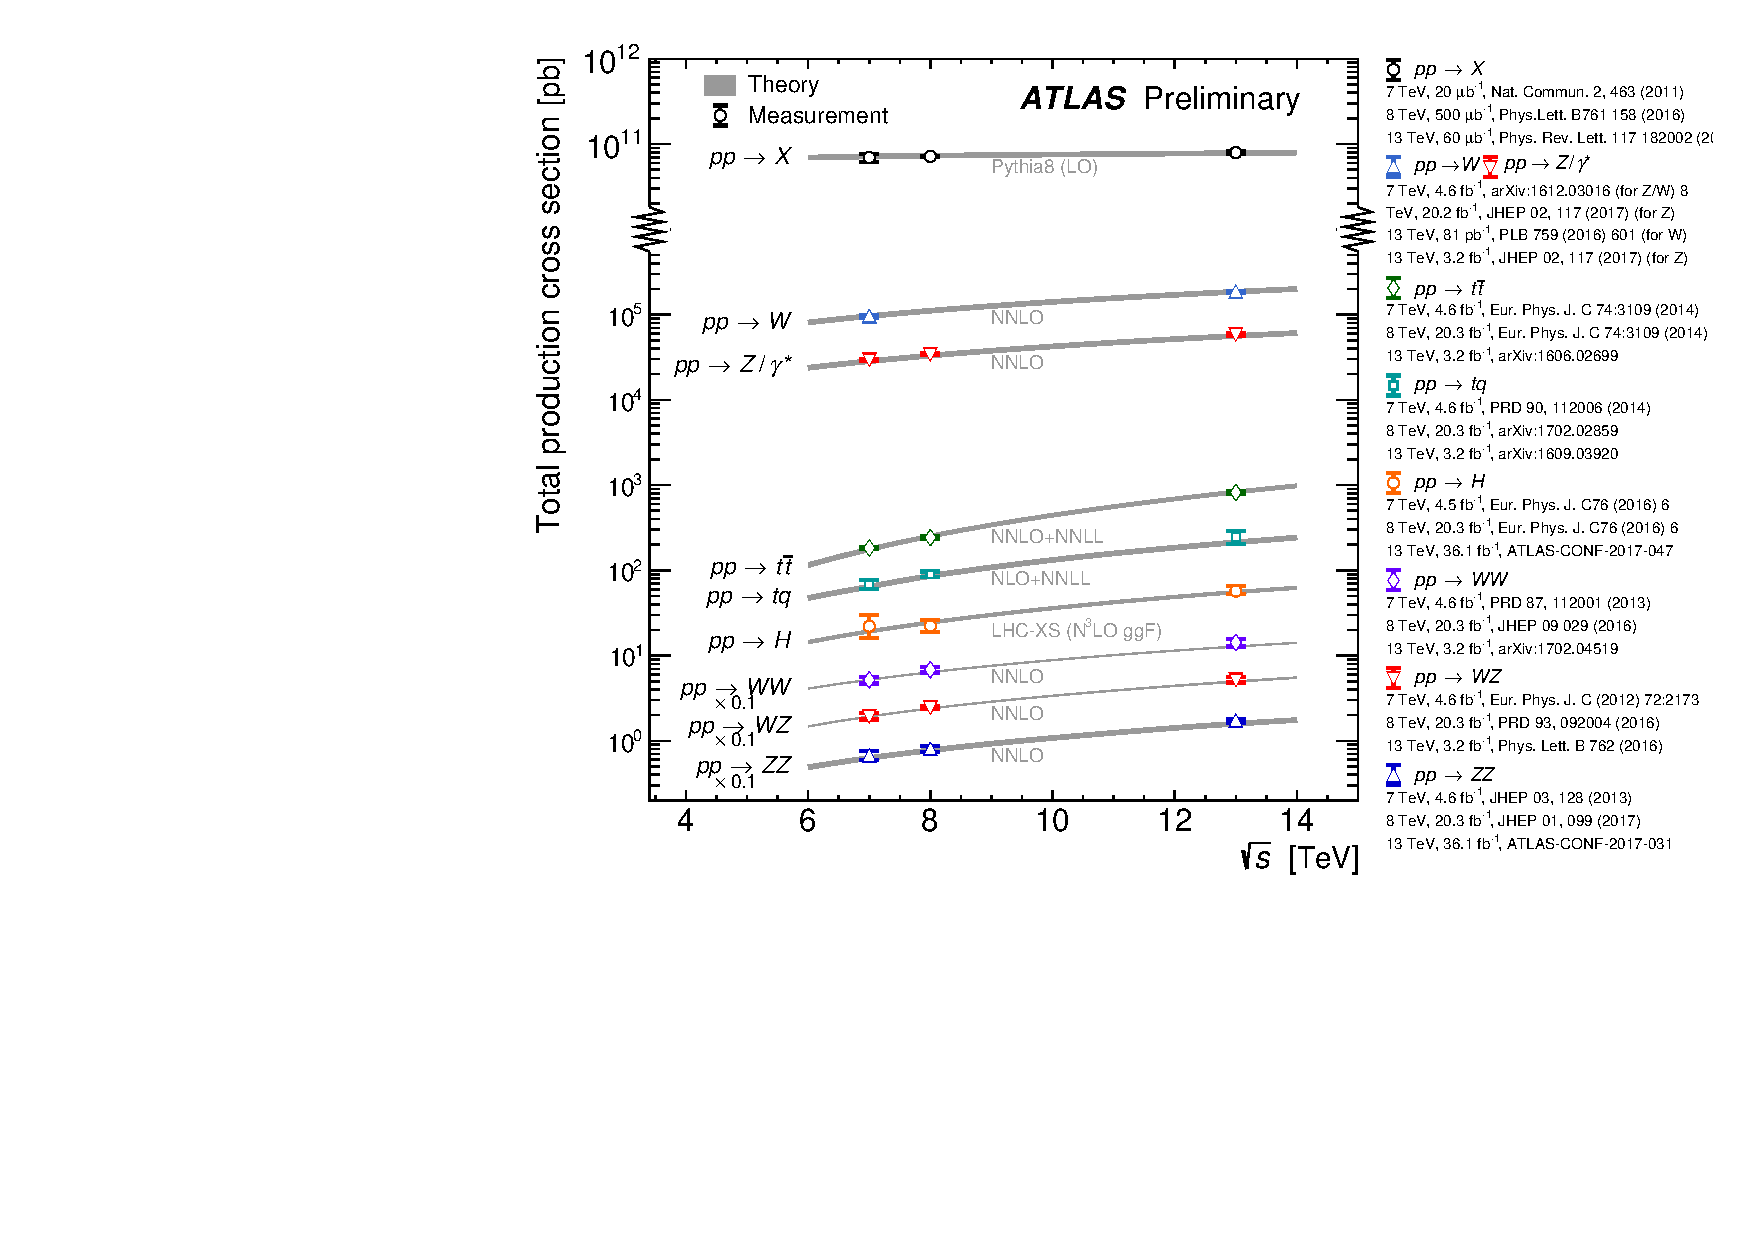
\includegraphics[width=0.7\textwidth]{figures/Theory/ATLAS_n_SMSummary_SqrtS.pdf}
  \caption{Total production cross-section presented by ATLAS as a function of centre-of-mass energy $\sqrt{s}$ from 7 to 13 TeV for some selected processes,
	   the diboson measurements are scaled by a factor 0.1 to allow a presentation without overlaps.}
  \label{fig:diboson_xs1}
\end{figure}

%% ======================================= Vector boson scattering ===================
\textbf{Vector boson scattering}

The $SU(2)_{L} \times U(1)_{Y}$ structure in SM predicts self-interactions between electroweak gauge bosons.
Those self-couplings can involve either three or four gauge bosons at a single vertex, known as triple gauge coupling (\textit{TGC}) and
quartic gauge couplings (\textit{QGC}), repectively.
Vector boson scattering or fusion (\textit{VBS} or \textit{VBF}) is carried out 
by four electroweak vector bosons, namely $Z$, $W^{\pm}$ and photon $(\gamma)$ as the Feynman diagrams shown in figure~\ref{fig:vbs_fd1}. 
And the vertexes include either those self-interactions
or the interactions with Higgs boson described in figure~\ref{fig:vbs_fd2}.
\begin{figure}[!htb]
  \centering
  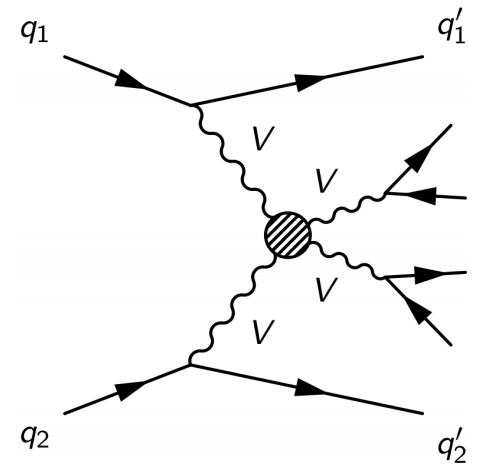
\includegraphics[width=0.4\textwidth]{figures/Theory/VBS.png} 
  \caption{Feynman disgrams of vector boson scattering.}
  \label{fig:vbs_fd1}
\end{figure}
\begin{figure}[!htb]
  \centering
  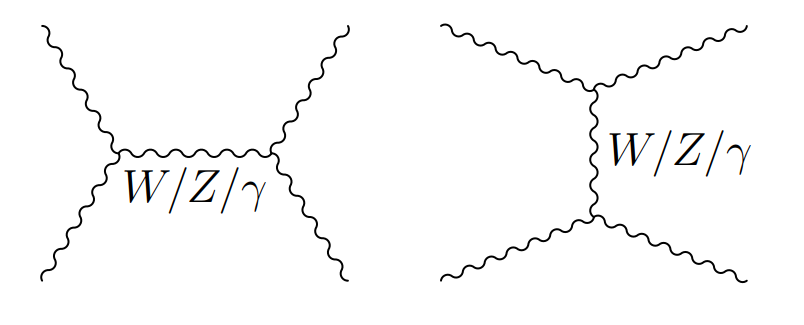
\includegraphics[width=0.6\textwidth]{figures/Theory/vbs_tgc.png} \\
  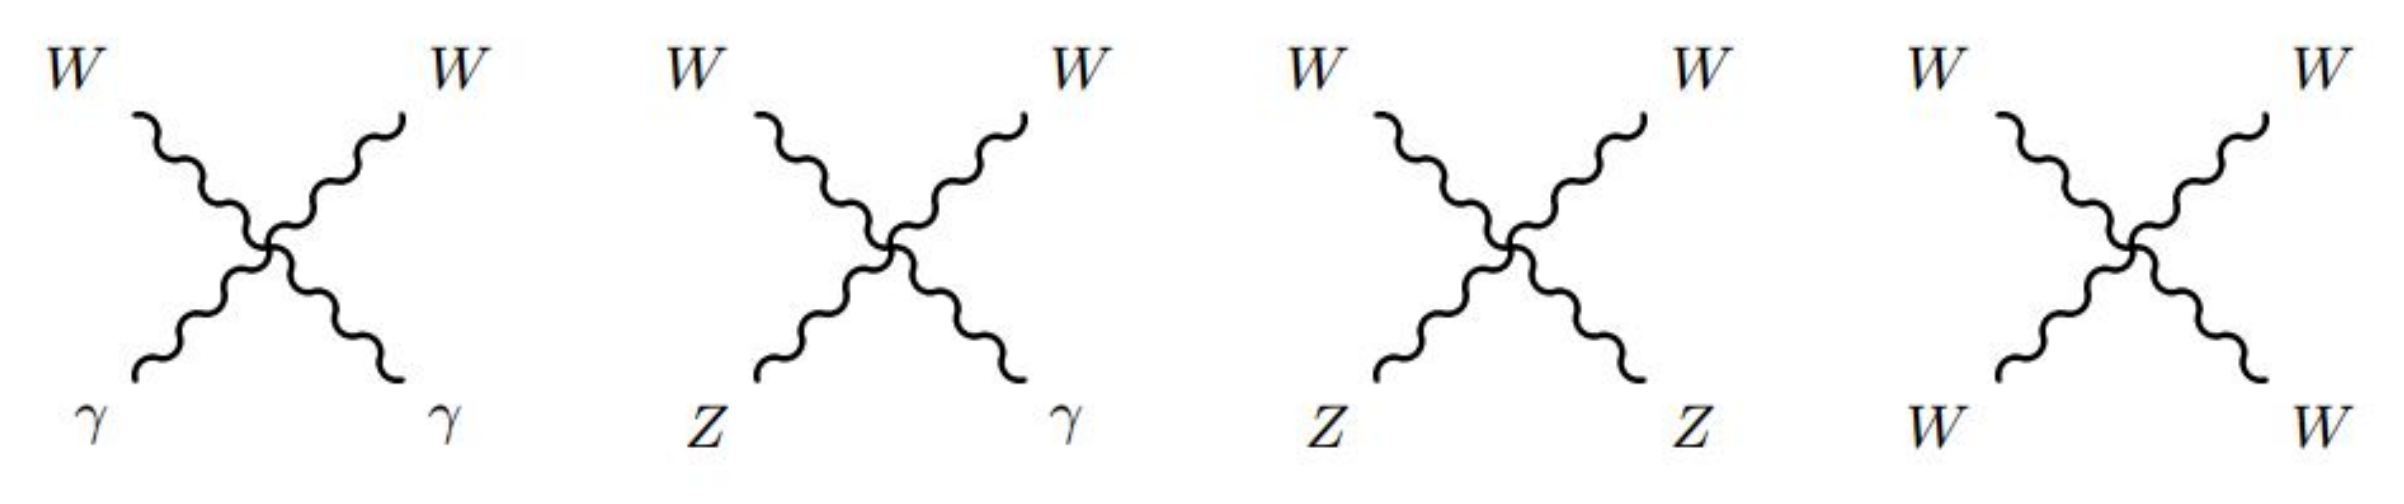
\includegraphics[width=1.0\textwidth]{figures/Theory/vbs_qgc.png} \\
  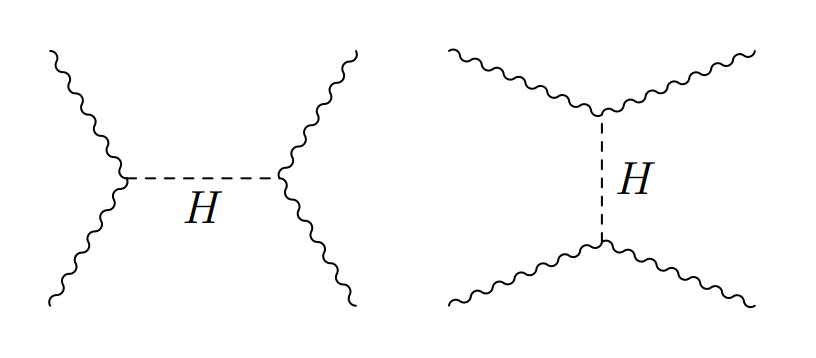
\includegraphics[width=0.6\textwidth]{figures/Theory/vbs_higgs.png} 
  %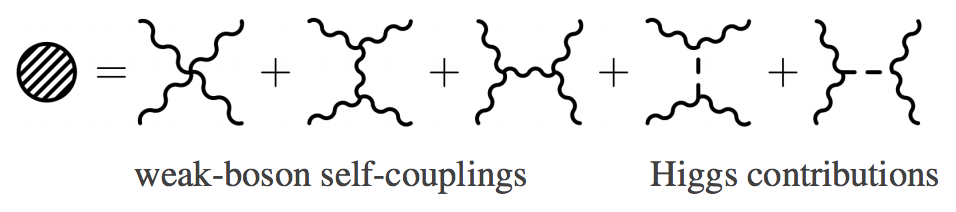
\includegraphics[width=1.0\textwidth]{figures/Theory/VBS_vertex.png}
  \caption{Feynman disgrams of vertexes involving QGC, TGC and Higgs.}
  \label{fig:vbs_fd2}
\end{figure}

The amplitudes of leading-order (LO) VBS can be expressed as:
\begin{equation} \label{eq:amp_tgc}
\begin{split}
	& {iM}_{TGC}^{s-channel} = -i\frac{g_{1}^{2}}{4m_{W}^{4}}[s(t-u)-3m_{W}^{2}(t-u)] \\
	& {iM}_{TGC}^{t-channel} = -i\frac{g_{1}^{2}}{4m_{W}^{4}}\left[t(s-u)-3m_{W}^{2}(s-u)+\frac{8m_{W}^{2}}{s}u^{2}\right]
\end{split}
\end{equation}
\begin{equation}
	{iM}_{QGC} = i\frac{g_{1}^{2}}{4m_{W}^{4}}\left[s^{2}+4st+t^{2}-4m_{W}^{2}(s+t)-\frac{8m_{W}^{2}}{s}ut\right]
\end{equation}
\begin{equation} \label{eq:amp_higgs}
\begin{split}
	{iM}_{Higgs} & = -i\frac{C_{\nu}^{2}g_{1}^{2}}{4m_{W}^{2}}\left[\frac{(s-2m_{W}^{2})^{2}}{s-m_{H}^{2}} + \frac{(t-2m_{W}^{2})^{2}}{t-m_{H}^{2}}\right] \\
                     & \simeq -i\frac{C_{\nu}^{2}g_{1}^{2}}{4m_{W}^{2}}(s+t)
\end{split}
\end{equation}
Combined s- and t-channel of TGC in Eq.~\ref{eq:amp_tgc}:
\begin{equation}
	{iM}_{TGC} = -i\frac{g_{1}^{2}}{4m_{W}^{4}}\left[s^{2}+4st+t^{2}+3m_{W}^{2}t-5m_{W}^{2}s+8m_{W}^{2}\frac{t^{2}}{s}\right]
\end{equation}
Then by combining the QGC term, the amplitude of self-couplings can be written as:
\begin{equation} \label{eq:self_coup}
	{iM}_{TGC} + {iM}_{QGC}= i\frac{g_{1}^{2}}{4m_{W}^{2}}(s+t) + {O}((s/m_{W}^{2})^{0})
\end{equation}
In Eq.~\ref{eq:self_coup}, the amplitude grows as a function of center-of-mass energy ($\sqrt{s}$),
which violates the unitarity in the TeV region.
Considering the Higgs term in Eq.~\ref{eq:amp_higgs} perfectly cancels out this growing,
and the remaining term ${O}((s/m_{W}^{2})^{0})$ depends on the total amplitude in SM.

In conclusion, Higgs boson acts as “moderator” to unitarize high-energy longitudinal vector boson scattering
by restoring unitarity of total amplitude in high energy region.

%\subsection{Diboson physics}
